\chapter{Utveckling av artificiell intelligens}
\label{sec:Deep}

I det följande kapitlet beskrivs utvecklingen av en artificiell intelligens baserad på djupinlärning med förmåga att förutsäga studieresultat i matematiktunga universitetskurser. Kapitlet inleds med en allmän introduktion till fältet djupinlärning. Introduktionen fördjupas med en beskrivning av kopplingarna mellan djupinlärning och osäkerheter, samt en kort bakgrund om korrelationsanalys. Därefter presenteras arbetets metod för att med djupinlärning förutsäga studieresultat. Till sist presenteras undersökningens resultat och en sammanfattande diskussion med en framåtblick mot vidare undersökningar.
\section{Bakgrund: artificiell intelligens och djupinlärning}
\label{sec:DeepBack}

Artificiell intelligens är ett samlingsbegrepp för metoder som automatiserar intellektuella uppgifter som vanligen utförs av människor \cite{Chollet}. Bland dessa metoder ingår maskin- och djupinlärning. I detta kapitel presenteras den grundläggande teorin bakom djupinlärning, samt hur djupinlärning kan kombineras med och analyseras av statistiska metoder. 

Djupinlärning är ett underfält till maskininlärning. Skillnaden mellan maskininlärning och klassisk programmering finns i vilken typ av problem de används till. Det klassiska programmeringsproblemet kan definieras som att utifrån indata $\mathbb{X}$ generera resultat $\mathbb{Y}$, genom att behandla indatan efter en fördefinierad sekvens av regler \cite{JavaGroundUp}. Det generella maskininlärningsproblemet kan definieras som att utifrån en indatamängd $\mathbb{X}$ finna en sannolikhetsfördelning $q\left(\mathbb{Y}|\mathbb{X}\right)$ som optimalt approximerar den sanna fördelningen $p\left(\mathbb{Y}|\mathbb{X}\right)$ \cite{variation}. Förenklat är målet att utifrån given data $\mathbb{X}$ finna en modell $q$ som sedan kan användas för att generera förutsägelser som stämmer väl överens med verkliga resultat $p$. I ordet maskininlärning kommer ''inlärningen'' från processen att finna modellen $q$. Processen kallas att träna ett maskininlärningssystem.


Vad som utmärker djupinlärning från andra former av maskininlärning är att inom djupinlärning utförs flera transformationer av indatan efter varandra, med förhoppning att varje transformation successivt ger en tydligare representation av indatan. Inom djupinlärning kallas det att nätverket lär sig flera lager av representation \cite{Chollet}. Dessa lager kan representeras med en struktur som kallas för ett \textit{neuralt nätverk}. Ett neuralt nätverk består av flera sammankopplade lager som motsvarar de olika lagren av representation, se figur \ref{fig:general_NN}. Det första lagret kallas indatalager, det sista utdatalager och lagren däremellan för dolda lager. Varje lager är i sin tur uppbyggt av flera noder. I ett tätt lager (eng. \emph{dense layer}) är varje nod sammankopplad med alla noder i det föregående lagret och i nästa lager, men inte i det egna lagret. Varje koppling mellan noder är skalad med en vikt $w$. Dessutom är varje nod associerad med ett förskjutningsvärde (eng. \emph{bias}) $b$. Transformationen mellan två noder $i$ och $j$ kan parametriseras av vikter och förskjutningsvärden på följande sätt 

\begin{equation}
    u_j = A \left(w_{ji}x_i + b_j\right),
    \label{eq:node_transform}
\end{equation}
där $x_i$ är indata till nod $j$ from nod $i$ och $u_j$ är utdata från nod $j$, se figur \ref{fig:general_NN}. $A$ kallas aktiveringsfunktion (eng. \emph{activation function}) \cite{Chollet}. På motsvarande sätt kan den totala transformationen för nod $i$:s lager uttryckas på matrisform som 

\begin{equation}
    \textbf{u} = A(\textbf{W} \cdot \textbf{x} + \textbf{b}),
    \label{eq:network_transform}
\end{equation}
\noindent där $\textbf{W}$ är en matris innehållande alla vikter mellan alla noder $i$ och $j$, $\textbf{x}$ är indatavektorn till lagret och \textbf{b} är en vektor som innehåller alla noders förskjutningsvärden. 

\begin{figure}[hbtp]
    \centering
    \resizebox {0.88\textwidth} {!} {
        \definecolor{input_node}{RGB}{171,171,154}
\definecolor{dense_node}{RGB}{196,225,144}
\definecolor{dropout_node}{RGB}{222,222,222}
\definecolor{output_node}{RGB}{171,154,154}
% New colors
\definecolor{klight_green_400}{RGB}{156, 204, 101}

\tikzset{%
  dense neuron/.style={
    circle,
    draw,
    fill=klight_green_400,
    thick,
    minimum size=0.75cm
  },
  dropout neuron/.style={
    circle,
    draw,
    fill=dropout_node,
    thick,
    minimum size=0.75cm
  },
  input neuron/.style={
    circle,
    draw,
    fill=input_node,
    thick,
    minimum size=0.75cm
  },
  output neuron/.style={
    circle,
    draw,
    fill=output_node,
    thick,
    minimum size=0.75cm
  },
  neuron missing/.style={
    draw=none, 
    scale=4,
    fill=none,
    text height=0.333cm,
    execute at begin node=\color{black}$\vdots$
  },
  zoom neuron/.style={
    circle,
    draw,
    fill=klight_green_400,
    opacity=0.3,
    minimum size=1.2cm
  },
  zoom line/.style={
    draw,
    opacity=0.3,
    line width=0.5mm,
    minimum size=1cm
  },
  z_connect line/.style={
    draw,
    line width=0.4mm,
    minimum size=1cm
  },
  highlight neuron/.style={
    circle,
    draw,
    fill=klight_green_400,
    minimum size=1.2cm
  },
  highlight line/.style={
    draw,
    opacity=1,
    line width=0.5mm,
    minimum size=1cm
  },
}

\begin{tikzpicture}[x=1.5cm, y=1.5cm, >=stealth]
\foreach \m/\l [count=\y] in {1,2,3,missing,4}
  \node [input neuron/.try, neuron \m/.try] (input-\m) at (0,2.5-\y) {};

\foreach \m [count=\y] in {1,missing,2}
  \node [dense neuron/.try, neuron \m/.try ] (hidden1-\m) at (1.5,2-\y*1.25) {};
  \foreach \m [count=\y] in {1,missing,2}
  \node [dense neuron/.try, neuron \m/.try ] (hidden2-\m) at (3,2-\y*1.25) {};

\foreach \m [count=\y] in {1,missing,2}
  \node [input neuron/.try, neuron \m/.try ] (output-\m) at (4.5,1.5-\y) {};

\foreach \l [count=\i] in {1,2,3,n}
  \draw [<-] (input-\i) -- ++(-1,0)
    node [above, midway] {\Large $x_\l$};

\foreach \l [count=\i] in {1,n}
  \draw [->] (output-\i) -- ++(1,0)
    node [above, midway] {\Large  $\hat{y}_\l$};

\foreach \i in {1,...,4}
  \foreach \j in {1,...,2}
    \draw [->] (input-\i) -- (hidden1-\j);
\foreach \i in {1,...,2}
  \foreach \j in {1,...,2}
    \draw [->] (hidden1-\i) -- (hidden2-\j);

\foreach \i in {1,...,2}
  \foreach \j in {1,...,2}
    \draw [->] (hidden2-\i) -- (output-\j);

\foreach \l [count=\x from 0] in {Indata-, Dolt tätt, Dolt tätt, Utdata-}
  \node [align=center, above] at (\x*1.5,2) {\l \\ lager};
  
  
% draw a box around zoom region

\draw[opacity=0.6, line width=0.3mm, dashed] ($(hidden1-1.north west)+(-0.4,0.4)$) rectangle ($(hidden2-2.south east)+(0.4,-0.4)$)
    node [] (box1) {}
    node (box2) at ($(hidden2-1.north east)+(+0.4,0.4)$)  {};



% ***** zoom

\foreach \m/\l [count=\y] in {1,2}
  \node [zoom neuron/.try, neuron \m/.try] (z_input-\m) at (7.5,5-\y*3-1) {};

\foreach \m [count=\y] in {1, 2}
  \node [zoom neuron/.try, neuron \m/.try ] (z_hidden1-\m) at (10.5,5-\y*3-1) {};


\foreach \l [count=\i] in {1,2}
  \draw [<-, zoom line/.try] (z_input-\i) -- ++(-1,0)
    node [above, midway] {};


\foreach \i in {1,...,2}
  \foreach \j in {1,...,2}
    \draw [->, zoom line/.try] (z_input-\i) -- (z_hidden1-\j);
    
% Mark certain nodes and corresponding lines
\node [highlight neuron/.try, neuron 1/.try ] (highlight-1) at (7.5,5-2*3-1) {\Large $i$};
\node [highlight neuron/.try, neuron 2/.try ] (highlight-2) at (10.5,5-1*3-1) {\Large $j$};
\node at (7.5+0.3,5-2*3-1+0.65) {\Large $x_{i}$};
\draw [->, highlight line/.try] (highlight-1) -- (highlight-2)
    node [] at (9, -0.1) {\Large $w_{ji}$};
\node at (10.5,5-1*3-1+0.65) {\Large $b_j$};
\draw [->, highlight line/.try] (highlight-2) -- ++(1,0)
    node [above, midway] {\Large $u_{j}$};
\draw [->, zoom line/.try] (z_hidden1-2) -- ++(1,0) {};

\draw[opacity=0.6, line width=0.25mm, dashed] ($(z_input-1.north west)+(-0.8,0.6)$) rectangle ($(z_hidden1-2.south east)+(0.8,-0.6)$)
    node (zoom1) at ($(z_input-2.south west)+(-0.8,-0.6)$) {}
    node (zoom2) at ($(z_input-1.north west)+(-0.8,0.6)$)  {};

% **** connect zoom and nn
\begin{scope}[->]
    \path[z_connect line/.try]
        (box1) edge[bend right] node [->, left] {} (zoom1)
        (box2) edge[bend left] node [->, left] {} (zoom2);
\end{scope}
\end{tikzpicture}
    }
    \caption{Ett neuralt nätverk bestående av ett indata-lager, två dolda täta lager och ett utdata-lager. ${x_1,...,x_n}$ och ${\hat{y_1},...,\hat{y_n}}$ är komponenter till indatan $\mathbb{X}$ respektive utdatan $\mathbb{\hat{Y}}$. Till höger visas en förstoring av de dolda täta lagren, med en schematisk skiss över hur två noder är kopplade till varandra. Notera att $x_i$ är utdata från nod $i$, $w_{ij}$ är viktningen av kopplingen mellan nod $i$ och $j$, $b_j$ är förskjutningsvärdet för nod $j$ och $u_j$ dess utdata. Parametrarna är relaterade enligt ekvation \eqref{eq:node_transform}.}
    \label{fig:general_NN}
\end{figure}

Träningen av det neurala nätverket består i att hitta dessa vikter $\textbf{W}$ och förskjutningsvärden $\textbf{b}$ för varje lager som ger den optimala modellen $q$ \cite{Chollet}. Den konventionella metoden för att åstadkomma detta är övervakad inlärning (eng. \emph{supervised learning}). Vid övervakad inlärning behövs träningsdata (eng. \emph{training data}) bestående av indata $\mathbb{X}_{tr}$ ihop med måldata $\mathbb{Y}_{tr}$ (eng. \emph{target data}). Om nätverkets utdata är $\mathbb{\hat{Y}}$ vid indata $\mathbb{X}_{tr}$ kan en förlustfunktion (eng. \emph{loss function}) $\mathcal{L}\left(\mathbb{\hat{Y}}, \mathbb{Y}_{tr} \right)$ definieras. Förlustfunktionen ger ett mått på hur väl måldatan $\mathbb{Y}_{tr}$ överensstämmer med nätverkets utdata $\mathbb{\hat{Y}}$. Förlustfunktionen kan sedan minimeras genom en process som kallas bakåtpropagation (eng. \emph{back propagation}) och utförs av en optimeringsfunktion, (eng. \emph{optimizer}).

% \begin{figure}[hbtp]
%     \centering
%     \resizebox {0.5\textwidth} {!} {
%         \definecolor{dense_node}{RGB}{196,225,144}
\definecolor{dropout_node}{RGB}{222,222,222}

\tikzset{%
  every neuron/.style={
    circle,
    draw,
    fill=dropout_node,
    opacity=0.3,
    minimum size=1cm
  },
  every line/.style={
    draw,
    opacity=0.3,
    minimum size=1cm
  },
  highlight neuron/.style={
    circle,
    draw,
    fill=dense_node,
    minimum size=1cm
  },
  highligh line/.style={
    draw,
    opacity=1,
    minimum size=1cm
  },
  neuron missing/.style={
    draw=none, 
    fill=none,
    scale=4,
    text height=0.333cm,
    execute at begin node=\color{black}$\vdots$
  },
}


\begin{tikzpicture}[x=1.5cm, y=1.5cm, >=stealth]

\foreach \m/\l [count=\y] in {1,2}
  \node [every neuron/.try, neuron \m/.try] (input-\m) at (0,2.5-\y*1.25) {};

\foreach \m [count=\y] in {1, 2}
  \node [every neuron/.try, neuron \m/.try ] (hidden1-\m) at (2,2.5-\y*1.25) {};

% \foreach \m/\l [count=\y] in {missing,1,2,missing}
%   \node [every neuron/.try, neuron \m/.try] (input-\m) at (0,2.5-\y*1.25) {};

% \foreach \m [count=\y] in {missing, 1, 2, missing}
%   \node [every neuron/.try, neuron \m/.try ] (hidden1-\m) at (2,2.5-\y*1.25) {};
  
% \foreach \m [count=\y] in {missing, 1, 2, missing}
%   \node [every neuron/.try, neuron \m/.try ] (hidden2-\m) at (4,2.5-\y*1.25) {};

% \foreach \m [count=\y] in {1}
%   \node [every neuron/.try, neuron \m/.try ] (output-\m) at (6,-2) {};

\foreach \l [count=\i] in {1,2}
  \draw [<-, every line/.try] (input-\i) -- ++(-1,0)
    node [above, midway] {};

% \foreach \l [count=\i] in {1,n}
%   \node [above] at (hidden-\i.north) {$H_\l$};

% \foreach \l [count=\i] in {j,j+1}
%   \draw [->, every line/.try] (hidden1-\i) -- ++(1,0)
%     node [above, midway] {$u_{\l}$};

\foreach \i in {1,...,2}
  \foreach \j in {1,...,2}
    \draw [->, every line/.try] (input-\i) -- (hidden1-\j);
    
% \foreach \i in {1,...,2}
%   \foreach \j in {1,...,2}
%     \draw [->, every line/.try] (hidden1-\i) -- (hidden2-\j);

% \foreach \i in {1,...,4}
%   \foreach \j in {1}
%     \draw [->, every line/.try] (hidden2-\i) -- (output-\j);

% \foreach \l [count=\x from 0] in {Indata-, Tätt, Tätt, Utdata-}
%   \node [align=center, above] at (\x*2,2) {\l \\ lager};

% Mark certain nodes and corresponding lines
\node [highlight neuron/.try, neuron 1/.try ] (highlight-1) at (0,2.5-2*1.25) {$i$};
\node [highlight neuron/.try, neuron 2/.try ] (highlight-2) at (2,2.5-1*1.25) {$j$};
\node at (2,2.5-1*1.25+0.5) {$b_j$};
\draw [->, highlight line/.try] (highlight-1) -- (highlight-2)
    node [above, midway] {$w_{ji}$};
\node at (0+0.5,2.5-2*1.25+0.1) {$x_{i}$};
\draw [->, highlight line/.try] (highlight-2) -- ++(1,0)
    node [above, midway] {$u_{j}$};
\draw [->, every line/.try] (hidden1-2) -- ++(1,0) {};

\end{tikzpicture}
%     }
%     \caption{En schematisk skiss över hur två noder är kopplade till varandra i ett neuralt nätverk. $x_i$ är utdata från nod $i$, $w_{ij}$ är viktningen av kopplingen mellan nod $i$ och $j$, $b_j$ är förskjutningsvärdet för nod $j$ och $u_j$ dess utdata. Dessa parametrar är relaterade enligt ekvation \eqref{eq:node_transform}.}
%     \label{fig:equation_transform}
% \end{figure}

För att förstå träningsprocessen och dess utmaningar inför vi begreppet \emph{generalisering}. Med generalisering menas hur väl ett tränat neuralt nätverks förutsägelser extrapolerar till annan data än träningsdatan. Generaliseringsgraden kan under träning uppskattas genom att låta nätverket utföra förutsägelser på valideringsdata (eng. \emph{validation data}). Valideringsdatan utgör en del av den tillgängliga datamängden som är skild från träningsdatan. Om valideringsdatan inte är oberoende av träningsdatan ges en felaktig bild av generaliseringsgraden, vilket kallas för kontaminering av valideringsdatan. Lägre prestanda på valideringsdatan än på träningsdatan är ett tecken på en vanligt förekommande utmaning som kallas överanpassning (eng. \emph{overfitting}). Överanpassning innebär att nätverket lär sig speciella mönster i träningsdatan som inte är generella för problemet. För att minimera överanpassning kommer vi använda oss av tre konventionella metoder: reducera nätverkets storlek, viktregularisation och utsläckning (eng. \emph{dropout}) \cite{Chollet}. Exempelvis innebär utsläckning att en viss del av indatan slumpvis sätts till noll vid en träningsomgång. Icke-generella mönster i datan kan därmed bli mindre tydliga, varav risken för överanpassning minskar.

En annan metod för att i allmänhet förbättra träningsprocessen av de neurala nätverken är normalisering av indatan \cite{Chollet}. Genom att transformera alla indataparametrar efter en normalfördelning med medelvärde $\mu = 0$ och standardavvikelse $\sigma = 1$, med andra ord en $\mathcal{N}(0,1)\text{-fördelning}$, blir storleken på parametrarna liknande. Nätverket behöver därmed inte under träning finna hur de olika parametrarna behöver skalas. För att undvika kontaminering av valideringsdatan beräknas medelvärdet $\mu_\mathrm{tr}$ och standardavvikelse $\sigma_\mathrm{tr}$ på träningsdatan $\mathbb{X}_{tr}$, varefter all indata $\mathbb{X}$ normaliseras enligt 

\begin{equation}
    \mathbb{X}_\mathrm{norm} = \frac{\mathbb{X}-\mu_\mathrm{tr}}{\sigma_\mathrm{tr}}.
    \label{normalization}
\end{equation}

Den färdigtränade modellen behöver även valideras och sättas i relation till verkligheten. En metod är att jämföra med en så kallad baslinje (eng. \emph{baseline}) för det aktuella problemet. En baslinje är prestandan som hade erhållits med en annan metod. Oftast väljs en enklare metod än ett neuralt nätverk \cite{Chollet}. Ett enkelt exempel är att försöka klassificera bilder på katter och hundar i en datamängd till 80\,\% bestående av katter. Om vi enbart klassificerar alla bilder som katter uppnår vi då en träffsäkerhet (eng. \emph{accuracy}) på 80\,\%, vilket är en möjlig baslinje för exempelproblemet.

I detta arbete kommer vi ställas mot tre klassiska maskininlärningsproblem: binär klassificering, flerklass-klassificering samt skalär regression. Binär klassificering och flerklass-klassificering innebär att klassificera indata i två respektive flera olika kategorier. Det skalära regressionsproblemet består i att förutsäga ett kontinuerligt värde utifrån indata \cite{Chollet}. I vårt fall är motsvarande problem att förutsäga studieresultaten: underkänt eller godkänt betyg, graderat betyg respektive skrivningspoäng. Vi kommer hädanefter kalla dessa problem för U/G-problemet, U/5-problemet respektive skrivningspoängsproblemet.

% Övergripande kan man se ett djupt neuralt nätverk som flera på varandra följande transformationer som omvandlar Ett exempel som Chollet tar upp för att visualisera detta är genom att tänka på hur man själv skulle separera två tillsammans ihopknycklade pappersbitar; genom att göra flera små, enkla rörelser kan till slut veckla ut pappersbitarna, och separarera dem. \cite{Chollet} 
\subsection{Djupa neurala nätverk och osäkerhet}
\label{NN_and_uncert}
Djupa neurala nätverk är utmärkta verktyg för att åstadkomma förutsägelser och klassificeringar. Ett exempel är bildigenkänningsalgoritmer, men dessa kan uppvisa opålitligheter vid introduktion av störningar \cite{Elephant}. Problemet kan förklaras utifrån designen av ett kanoniskt klassfieringsproblem eftersom den tvingar det neurala nätverket att utföra en specifik klassificering. Detta leder i sin tur till översäkra neurala nätverk \cite{Kendall-Gal}. En möjlig lösning till problemet är att kombinera klassificeringen med en modell för osäkerhet. Detta kan åstadkommas med exempelvis bayesianska neurala nätverk (eng. \emph{Bayesian Neural Networks}) \cite{Kendall-Gal} eller genom att modifiera förlustfunktionerna för att bygga in en uppskattning av osäkerheter.

För att underlätta förståelsen av osäkerheter i modellerna introducerar vi begreppen \emph{epistemisk osäkerhet} \cite{Uncert} och \emph{aleatorisk osäkerhet} \cite{Uncert}. Epistemisk osäkerhet kan tolkas som modellosäkerhet medan aleatorisk osäkerhet kan tolkas som en intrinsisk osäkerhet i indatan. Osäkerheterna kan även uttryckas i termer som är specifika för neurala nätverk. Betrakta ett neuralt nätverk $f^\mathbf{W}$ vars vikter och förskjutningsvärden gemensamt symboliseras av $\mathbf{W}$, och med indatamängd $\mathbb{X}_{tr} = \{\mathbf{x_1},..., \mathbf{x_n}\}$ som avbildar $\mathbf{x_i}$ på förutsägelse $\hat{y}_i = f^\mathbf{W}(\mathbf{x}_i)$ som en uppskattning av utdatamängden $\mathbb{Y}_{tr} = \{y_1,..., y_n\}$. Det är möjligt utifrån det neurala nätverket som modell att identifiera tre former av osäkerheter i form av aleatorisk indataosäkerhet $\sigma_x$, epistemisk viktosäkerhet $\sigma_W$ och förutsägelseosäkerhet $\sigma_y$.

Det huvudsakliga problemet för att kvantifiera osäkerheter i neurala nätverk är att bestämma en funktion $U$ som utifrån $\sigma_x$ och $\sigma_W$ approximerar osäkerheten i förutsägelse $\sigma_y = U(\sigma_x, \sigma_W)$. Förslagsvis kan $\sigma_W$ uppskattas med bayesiansk djupinlärning (eng. \emph{Bayesian Deep Learning}) \cite{Kendall-Gal} och $\sigma_x$ genom att modifiera vanligt förekommande förlustfunktioner \cite{Kendall-Gal}. Emellertid kräver bayesiansk djupinlärning stora mängder beräkningskraft varför approximativa lösningar behöver tillämpas \cite{MC-dropout}. Därav väljer vi för det här arbetet att avgränsa ifrån bayesiansk djupinlärning och epistemisk osäkerhet för att istället fokusera på den aleatoriska osäkerheten i indata. Dessutom avgränsar vi undersökningen till införandet av aleatorisk osäkerhet för skrivningspoängsproblemet då det problemet gör implementationen så enkel som möjligt.

I Appendix \ref{app: derivation} visar vi hur aleatorisk osäkerhet $\sigma_x$ kan implementeras i förlustfunktioner och därigenom uppskattas av neurala nätverk. Under antagande att utdatan är normalfördelad givet indatan är förlustfunktionen
\begin{equation}
    \mathcal{L}_{\mathrm{normal}}(\mathbf{W}) = \exp{\left(-\log \sigma_x^2 \right)} \left\|y - f^\mathbf{W}(\mathbf{x})\right\|_2 + \log \sigma_x^2.
    \label{eq:loss_fcn}
\end{equation}
Speciellt kan det noteras att för konstant $\sigma_x^2$ återfås den kanoniska kvadratiska förlustfunktionen (eng. \emph{Mean Squared Error}, MSE) $\mathcal{L}_\mathrm{MSE}(\mathbf{W}) = \left\|y - f^\mathbf{W}(\mathbf{x})\right\|_2$. Jämfört med den kvadratiska förlustfunktionen medför den aleatoriska osäkerheten en osäkerhetsattenuationsfaktor $\exp{\left(-\log \sigma_x^2 \right)}$ som minskar bidraget av felet $\left\|y - f^\mathbf{W}(\mathbf{x})\right\|_2$ vid växande osäkerheter $\sigma_x$. Dessutom införs en osäkerhetsterm $\log \sigma_x^2$ som bidrar växande till förlustfunktionen för växande $\sigma_x^2$.

\subsection{Korrelationer för analys av indata}
\label{sec:korre}
Kvaliteten på förutsägelserna $\hat{y}_i = f^\mathbf{W}(\mathbf{x}_i)$ från ett neuralt nätverk påverkas i stor utsträckning av hur väl indatan $\mathbb{X}$ faktiskt kopplar till måldatan $\mathbb{Y}$. Ett statistiskt verktyg för att analysera kopplingen mellan $\mathbb{X}$ och $\mathbb{Y}$ är korrelationskoefficienter. En korrelationskoefficient är ett mått på hur mycket två variabler korrelerar linjärt med varandra. Den vanligaste varianten är Pearsons korrelationskoefficient. Låt $\mathbf{x}$ och $\mathbf{y}$ vara två vektorer. Då definieras Pearsons korrelationskoefficient som \cite{ProbStat}

\begin{equation}
    \rho_{\mathbf{x},\mathbf{y}} = \frac{\text{cov}(\mathbf{x,y})}{\sigma_\mathbf{x}\sigma_\mathbf{y}},
\end{equation}

\noindent
där $\text{cov}(\mathbf{x,y})$ står för kovariansen mellan $\mathbf{x}$ och $\mathbf{y}$ medan $\mathbf{\sigma}_\mathbf{x} \, (\mathbf{\sigma}_\mathbf{y}$) är standardavvikelsen för $\mathbf{x} \, (\mathbf{y}$). Koefficienten $\rho_{\mathbf{x},\mathbf{y}} \in [-1,1]$, där -1 betyder en stark negativ korrelation och 1 en stark positiv korrelation. Två variabler är okorrelerade om $\rho_{\mathbf{x},\mathbf{y}} = 0$. 

För att kunna få fram hur $n$ variabler är linjärt korrelerade med en variabel används multikorrelation (eng. \emph{multi correlation}). Multikorrelation ger ett mått på hur väl en given variabel kan förutsägas med hjälp av en linjär funktion av $n$ andra variabler. Låt $\mathbf{x}_{i}$ för $i = 1, 2, ..., n$ vara indatavektorerna vi använder oss av för att förutsäga utdatavektorn $\mathbf{y}$. Beteckna $R^2$ som kvadraten på vår multikorrelation, definierad som \cite{multikorr}

\begin{equation}
    R^{2} = \mathbf{c}^{T}R_{xx}^{-1}\mathbf{c},
    \label{eq:multikorre}
\end{equation}

\noindent
där $\mathbf{c} = (\rho_{\mathbf{x}_1\mathbf{y}}, \rho_{\mathbf{x}_2\mathbf{y}}, ..., \rho_{\mathbf{x}_n\mathbf{y}})$. $R_{\mathbf{xx}}$ är en matris där varje element är en korrelation mellan två $\mathbf{x}_i$. 

 
\begin{equation}
    R_{\mathbf{xx}} = 
    \begin{bmatrix}
    \rho_{\mathbf{x}_1\mathbf{x}_1} & \rho_{\mathbf{x}_1\mathbf{x}_2} &  \dots  & \rho_{\mathbf{x}_1\mathbf{x}_n} \\
    \rho_{\mathbf{x}_2\mathbf{x}_1} & \rho_{\mathbf{x}_2\mathbf{x}_2} & \dots  & \rho_{\mathbf{x}_2\mathbf{x}_n} \\
    \vdots & \vdots  & \ddots & \vdots \\
    \rho_{\mathbf{x}_n\mathbf{x}_1} & \rho_{\mathbf{x}_n\mathbf{x}_2} & \dots  & \rho_{\mathbf{x}_n\mathbf{x}_n}
\end{bmatrix}.    
\end{equation}

\noindent
Matrisen $R_\mathbf{xx}$ ger ett mått på hur variablerna $\mathbf{x}_{i}$ korrelerar med varandra. Om alla dessa variabler är okorrelerade kommer $R_\mathbf{xx} = I$, där $I$ symboliserar identitetsmatrisen. Detta resulterar i att $R^2$ blir summan av korrelationer mellan variabel $\mathbf{x}_{i}$ och $\mathbf{y}$ i kvadrat, det vill säga $R^2 = \mathbf{c}^{T}\mathbf{c} = \sum_i \rho_{x_i,y}^2$.

\section{Metod}
Med utgångspunkt i bakgrunden ovan presenterar vi härnäst vår metod för att med djupinlärning förutsäga studieresultat. I avsnittet beskrivs inledningsvis datan och dataanalysen som utvecklingen grundas på. Därefter presenterar vi hur vi har tränat och validerat våra neurala nätverk. Dessutom beskrivs arkitekturerna för nätverken med högst validerad prestanda, och en felanalys av deras förutsägelser. 

\subsection{Databeskrivning, databehandling och dataanlys}
\label{sec:DDD}

%I det här avsnittet presenteras hur den tillgängliga datan har behandlats till en form som lämpar sig för de neurala nätverken. Först ges en beskrivning av rådatan, följt av hur den har omformaterats och processats. Sist ges en beskrivning av hur datan har analyserats. 





%\begin{figure}[hbtp]
% \begin{center}
%    \resizebox {0.5\textwidth} {!} {
%       \definecolor{klight_green_400}{RGB}{156, 204, 101}
\definecolor{YATA_green}{RGB}{112, 181, 1}
\definecolor{Google_Red}{RGB}{231,69,60}

\newcommand\widthx{4}
\newcommand\heighty{4}



\begin{tikzpicture}[x=0.25cm, y=0.25cm, ->,>=stealth',auto, thick] 

\tikzset{%
  data part/.style={
    rectangle,
    %Change fill for draw if you want boarders
    fill,
    text=white,
    opacity=0.5,
    fill=klight_green_400,
    thick,
    minimum width=2cm,
    minimum height=2cm
  },
  text part/.style={
    opacity=1,
    text=black,
    text height=0.25cm,
  },
  text2 part/.style={
    opacity=1,
    text=black,
    rotate=65,
  },
}

% User squared
%\node [data part/.try] (layer2) at (4,4) {};
\node [data part/.try] (layer2) at (3,3) {};
\node [data part/.try] (layer2) at (2,2) {};
\node [data part/.try] (layer2) at (1,1) {};
\node [data part/.try] (layer1) at (0,0) {};

% Home made axis
\draw (-4.5,4.5) -- (4,4.5);
\draw (-4.5,4.5) -- (-4.5,-4.5);
\draw[color=Google_Red] (-4.5,4.5) -- (0,9);

% Name of axies
\node[text part/.try] at (1.25,5.25) {\small $\textbf{Egenskaper}$};
\node[text part/.try, rotate=45] at (-2.75,7.75) {\small $\textbf{Studenter}$};
\node[text part/.try, rotate=90] at (-5.5,0) {\small $\textbf{Uppgifter}$};

% 3 boxes per line
%\draw [dashed, color=YATA_green, -] (-4,1.5) -- (4,1.5);
%\draw [dashed, color=YATA_green, -] (-4,-1.5) -- (4,-1.5);
%\draw [dashed, color=YATA_green, -] (-1.5,-4) -- (-1.5,4);
%\draw [dashed, color=YATA_green, -] (1.5,-4) -- (1.5,4);

% 4 boxer per line
%\draw [dashed, color=YATA_green, -] (-4,2) -- (4,2);
%\draw [dashed, color=YATA_green, -] (-4,0) -- (4,0);
%\draw [dashed, color=YATA_green, -] (-4,-2) -- (4,-2);

%\draw [dashed, color=YATA_green, -] (-2,4) -- (-2,-4);
%\draw [dashed, color=YATA_green, -] (0,4) -- (0,-4);
%\draw [dashed, color=YATA_green, -] (2,4) -- (2,-4);

\draw [dashed, color=YATA_green, -] (-4,2.4) -- (4,2.4);
\draw [dashed, color=YATA_green, -] (-4,0.8) -- (4,0.8);
\draw [dashed, color=YATA_green, -] (-4,-0.8) -- (4,-0.8);
\draw [dashed, color=YATA_green, -] (-4,-2.4) -- (4,-2.4);

\draw [dashed, color=YATA_green, -] (-2.4, 4) -- (-2.4,-4);
\draw [dashed, color=YATA_green, -] (-0.8,4) -- (-0.8,-4);
\draw [dashed, color=YATA_green, -] (0.8,4) -- (0.8,-4);
\draw [dashed, color=YATA_green, -] (2.4,4) -- (2.4,-4);







% Connect them 
\path[main line/.style={font=\sffamily\small}];
    % YATA Flow
    %(YATA) edge node [left] {} (YATAData)

    
\end{tikzpicture}
%   }
%  \end{center}
%  \caption{Lorem ipsum.}
%  \label{fig:tensor}
% end{figure}




% Grönt indikerar de steg som datan genomgår under formateringen till tensorer, och grått indikerar de processer som behandlar datan.

För arbetet omfattade den totala datamängden rådata från tre olika kurser på Chalmers tekniska högskola: FFM521 (Mekanik 2 år 2017), FFM234 (Vektorfält och klassisk fysik år 2018) samt TMS064 (Matematisk statistik år 2019). För att förenkla notationen kallar vi hädanefter FFM521 för kurs A, FFM234 för kurs B och TMS064 för kurs C. Rådatan från kurs A och B var anonymiserad och samlades in via applikationen OpenTA. Den bestod av tidsserier från 151 respektive 101 studenter. Rådatan från kurs C samlades in via den av oss utvecklade webbsidan YATA och utgjordes av tidsserier från 17 studenter. Se appendix \ref{app: dataDescription} för en mer detaljerad beskrivning av rådatan. Inom fältet djupinlärning utgör de cirka 300 studenterna en liten datamängd \cite{Chollet}. Tidsserierna utgjordes av en sekvens av rader där varje rad uppkom när en student gjorde ett försök på en uppgift. En rad bestod av fyra attribut: anonymiserat student-ID, uppgifts-ID, om studentens försök på uppgiften var korrekt och tidpunkt för försöket. Till OpenTA-datan fanns även tillhörande tentamensresultat från ordinarie skrivningstillfälle. Betygsfördelningen för kurs A var U: 59\,\%, 3: 30\,\%, 4: 7.2\,\% och 5: 3.3\,\%, avrundat till två värdesiffror. Betygsfördelningen för kurs B var U: 46\,\%, 3: 32\,\%, 4: 17\,\% och 5: 5.9\,\%. För kurs C fanns inte tillhörande tentamensresultat eftersom kursen pågick under arbetets gång. På grund av att tentamensresultat var tillgängliga för kurs A och B användes datan från dem för att undersöka om det var möjligt att förutsäga studieresultat, medan datan från kurs C användes för att undersöka interaktionen mellan student och artificiell intelligens.

\begin{wrapfigure}{r}{0.38\textwidth}
  \begin{center}
    \resizebox {0.38\textwidth} {!} {
        \definecolor{input_node}{RGB}{171,171,154}
\definecolor{dense_node}{RGB}{196,225,144}
\definecolor{dropout_node}{RGB}{222,222,222}
\definecolor{output_node}{RGB}{171,154,154}
% New colors
\definecolor{klight_green_400}{RGB}{156, 204, 101}
\definecolor{YATA_green}{RGB}{112, 181, 1}



\begin{tikzpicture}[x=6cm, y=2.5cm, ->,>=stealth',auto, thick] 
\tikzset{%
  data part/.style={
    rectangle,
    draw,
    text=white,
    fill=klight_green_400,
    thick,
    minimum width=4cm,
    minimum height=1.2cm
  },
  platform part/.style={
    rectangle,
    draw,
    fill=output_node,
    thick,
    text=white,
    minimum width=5cm,
    minimum height=1.2cm
  },
  process part/.style={
    rectangle,
    draw,
    fill=dropout_node,
    thick,
    minimum width=5cm,
    minimum height=1.2cm
  },
  analysis part/.style={
    rectangle,
    draw,
    fill=YATA_green,
    thick,
    text=white,
    minimum width=3cm,
    minimum height=1.5cm
  },
  main line/.style={
    draw,
    line width=0.25mm,
    opacity=1,
    minimum size=1cm
  },
  data line/.style={
    draw,
    line width=0.25mm,
    fill=klight_green_400,
    opacity=1,
    minimum size=1cm
  }
}
% Column 1
\node [data part/.try] (OpenData) at (0.1,1) {\Large \textbf{OpenTA}};
%\node [process part/.try] (OpenFormat) at (0,0){\Large $\textbf{Formatera OpenTA}$};

% Column 2
%\node [process part/.try] (YATAFormat) at (1,0) {\Large $\textbf{Formatera YATA}$};
\node [data part/.try] (YATAData) at (0.9,1) {\Large \textbf{YATA}};
%\node [platform part/.try] (YATA) at (1,2) {\Large $\textbf{YATA}$};

% Column 1.5
\node [process part/.try] (Formaterare) at (0.5,0) {\Large $\textbf{Formaterare}$};
\node [data part/.try] (DataFormat) at (0.5,-1) {\Large $\textbf{Formaterad data}$};
%\node [process part/.try] (TensorFormat) at (0.5,-2) {\Large $\textbf{Formatera Tensor}$};
\node [process part/.try] (TensorGen) at (0.5,-2) {\Large $\textbf{Generera tensor}$};
\node [data part/.try] (Tensor) at (0.5,-3) {\Large $\textbf{Tensor}$};
\node [analysis part/.try, align=center] (Stat) at (-0.2,-3) {\Large     \textbf{Data-} \\ \Large                                                                            \textbf{analys}};
\node [platform part/.try] (NN) at (0.5,-6) {\Large $\textbf{Neurala Nätverk}$};
\node [process part/.try] (Norm) at (0.5,-4) {\Large $\textbf{Normalisering}$};
\node [data part/.try] (NormTens) at (0.5,-5) {\Large $\textbf{Normaliserad Tensor}$};



%\node [project part/.try] (Egen) at (-0.5,-1) {$\textbf{Egenskaps selektion}$};
%node [project part/.try] (collect) at (2,2) {$\textbf{Analys}$};
%\node [project part/.try] (concept) at (0,0) {$\textbf{Koncept}$};
%\node [project part/.try] (use) at (4,0) {$\textbf{Användning}$};
%\node [project part/.try] (implement) at (2,-2) {$\textbf{Implementation}$};


% Connect them 
\path[main line/.style={font=\sffamily\small}]
    % YATA Flow
%    (YATA) edge node [left] {} (YATAData)
    (YATAData) edge node [left] {} (Formaterare)
    %(YATAFormat) edge node [left] {} (DataFormat)
    
    % OpenTA flow
    (OpenData) edge node [left] {} (Formaterare)
    %(OpenFormat) edge node [left] {} (DataFormat)
    
    % Tensorflow
    (Formaterare) edge node [left] {} (DataFormat)
    (DataFormat) edge node [left] {} (TensorGen)
    %(TensorFormat) edge node [left] {} (TensorGen)
    (TensorGen) edge node [left] {} (Tensor)
    (Tensor) edge node [left] {} (Norm)
    (Tensor) edge node [left] {} (Stat)
    (Stat) edge[bend right=-25] node [left] {} (TensorGen)
    
    (Norm) edge node [left] {} (NormTens)
    (NormTens) edge node [left] {} (NN);
    
    %(Stat) edge node [left] {} (Egen)
    %(Egen) edge node [left] {} (TensorFormat)
\end{tikzpicture}
    }
  \end{center}
  \caption{Ett flödesdiagram över databehandlings- och analysmetodiken. Notera att genereringen av tensorn är återkopplad via dataanalys.}
  \label{fig:dataflow}
\end{wrapfigure}

Neurala nätverk behöver indata och måldata, vilket beskrevs i sektion \ref{sec:DeepBack}. Som indata användes den insamlade datan för kurs A, B och C och som måldata i kurs A och B användes motsvarande tentamensresultat. Indata är konventionellt på tensorform \cite{Chollet} varav rådatan behöver transformeras. Transformationen av rådatan till tensorer bestod av tre moment och beskrivs i figur \ref{fig:dataflow}. I det första momentet omformaterades rådatan från de olika källorna till ett enhetligt format. Omformateringen krävdes på grund av att formatet på rådatan från OpenTA och YATA var olika. I det andra momentet genererades tredimensionella tensorer med axlar: unik student, unika uppgifter respektive egenskaper (eng. \textit{features}). Se figur \ref{fig:tensor} för en grafisk representation av tensorn. Fem kandidater till egenskaper extraherades från den omformaterade rådatan. Egenskaperna var: om studenten löste uppgiften, antal försök på uppgiften, tidpunkt i kursen då uppgiften påbörjades, medeltid mellan försök på uppgiften samt total tid spenderad på uppgiften. Enheten för tid valdes till sekunder. Om studenten inte påbörjade en uppgift sattes ett förvalt värde på de tidsrelaterade egenskaperna för den uppgiften som motsvarade total kurstid. De fem egenskaperna valdes ut då de relativt enkelt kunde extraheras ur rådatan.

För att verifiera att de fem kandidaterna till egenskaper var lämpliga som indata till nätverken utfördes en dataanalys. I dataanalysen beräknades korrelationskoefficienter för varje egenskap i kurs A och B mot tentamensresultaten. Beräkningarna utfördes genom att först summera över uppgifterna för varje egenskap för att erhålla ett totalt värde per egenskap. Korrelationskoefficienterna beräknades därefter på de totala värdena. Korrelationerna för egenskaperna kompletterades med multikorrelationskoefficienter för alla egenskaper tillsammans vilka beräknades enligt ekvation \eqref{eq:multikorre}. Multikorrelationerna användes i syfte att undersöka vad den sammanlagda korrelationen var mellan alla egenskaper och tentamensresultatet. Eventuella egenskaper med korrelationskoefficienter mindre än 0.25 bedömdes som svagt korrelerade \cite{ProbStat} och exkluderades i så fall från de slutgiltiga tensorerna. 


\begin{wrapfigure}{r}{0.32\textwidth}
    \centering
    \resizebox {0.32\textwidth} {!} {
        \definecolor{klight_green_400}{RGB}{156, 204, 101}
\definecolor{YATA_green}{RGB}{112, 181, 1}
\definecolor{Google_Red}{RGB}{231,69,60}

\newcommand\widthx{4}
\newcommand\heighty{4}



\begin{tikzpicture}[x=0.25cm, y=0.25cm, ->,>=stealth',auto, thick] 

\tikzset{%
  data part/.style={
    rectangle,
    %Change fill for draw if you want boarders
    fill,
    text=white,
    opacity=0.5,
    fill=klight_green_400,
    thick,
    minimum width=2cm,
    minimum height=2cm
  },
  text part/.style={
    opacity=1,
    text=black,
    text height=0.25cm,
  },
  text2 part/.style={
    opacity=1,
    text=black,
    rotate=65,
  },
}

% User squared
%\node [data part/.try] (layer2) at (4,4) {};
\node [data part/.try] (layer2) at (3,3) {};
\node [data part/.try] (layer2) at (2,2) {};
\node [data part/.try] (layer2) at (1,1) {};
\node [data part/.try] (layer1) at (0,0) {};

% Home made axis
\draw (-4.5,4.5) -- (4,4.5);
\draw (-4.5,4.5) -- (-4.5,-4.5);
\draw[color=Google_Red] (-4.5,4.5) -- (0,9);

% Name of axies
\node[text part/.try] at (1.25,5.25) {\small $\textbf{Egenskaper}$};
\node[text part/.try, rotate=45] at (-2.75,7.75) {\small $\textbf{Studenter}$};
\node[text part/.try, rotate=90] at (-5.5,0) {\small $\textbf{Uppgifter}$};

% 3 boxes per line
%\draw [dashed, color=YATA_green, -] (-4,1.5) -- (4,1.5);
%\draw [dashed, color=YATA_green, -] (-4,-1.5) -- (4,-1.5);
%\draw [dashed, color=YATA_green, -] (-1.5,-4) -- (-1.5,4);
%\draw [dashed, color=YATA_green, -] (1.5,-4) -- (1.5,4);

% 4 boxer per line
%\draw [dashed, color=YATA_green, -] (-4,2) -- (4,2);
%\draw [dashed, color=YATA_green, -] (-4,0) -- (4,0);
%\draw [dashed, color=YATA_green, -] (-4,-2) -- (4,-2);

%\draw [dashed, color=YATA_green, -] (-2,4) -- (-2,-4);
%\draw [dashed, color=YATA_green, -] (0,4) -- (0,-4);
%\draw [dashed, color=YATA_green, -] (2,4) -- (2,-4);

\draw [dashed, color=YATA_green, -] (-4,2.4) -- (4,2.4);
\draw [dashed, color=YATA_green, -] (-4,0.8) -- (4,0.8);
\draw [dashed, color=YATA_green, -] (-4,-0.8) -- (4,-0.8);
\draw [dashed, color=YATA_green, -] (-4,-2.4) -- (4,-2.4);

\draw [dashed, color=YATA_green, -] (-2.4, 4) -- (-2.4,-4);
\draw [dashed, color=YATA_green, -] (-0.8,4) -- (-0.8,-4);
\draw [dashed, color=YATA_green, -] (0.8,4) -- (0.8,-4);
\draw [dashed, color=YATA_green, -] (2.4,4) -- (2.4,-4);







% Connect them 
\path[main line/.style={font=\sffamily\small}];
    % YATA Flow
    %(YATA) edge node [left] {} (YATAData)

    
\end{tikzpicture}
    }
    \caption{En grafisk representation av den tredimensionella tensorn. Notera att användaraxeln (röd pil) utgjorde summationsriktning vid normalisering av tensorn. }
    \label{fig:tensor}
\end{wrapfigure}

%TODO: 1. Normalisering. 2. Beskrivning av implementationen. 

I det tredje momentet av databehandlingen normaliserades tensorerna med de utvalda egenskaperna från dataanalysen. De extraherade värdena för respektive egenskap i tensorn normaliserades uppgiftsvis för varje egenskap till en $\mathcal{N}(0,1)$-fördelning enligt ekvation \eqref{normalization}. Motsvarande måldata erhölls genom normering av tentamensresultaten för alla studenter. Tentamensresultaten representerades på olika sätt för vart och ett av de tre problemen. Måldatan för U/G-problemet var binär 0 eller 1, där 0 motsvarade underkänt och 1 godkänt. För U/5-problemet representerades måldatan av en ett-noll-kodning (eng. \emph{one-hot encoding}) av betygen och för skrivningspoängsproblemet utgjordes måldatan av de direkta skrivningspoängen.


Databehandlingen och dataanalysen implementerades i Python. Huvudsakligen användes databehandlingspaketen Pandas och Numpy för att processa datan. Paketen användes på grund av ökad kontroll över dataflödet och möjligheten att skala databehandlingen med antalet studenter som använder webbsidan YATA. Dessutom möjliggör paketen för mer avancerad dataanalys i framtiden.

\subsection{Träning och validering av neurala nätverk}
\label{sec:training_and_validation}
Här presenteras metoder som har använts för att generellt utveckla, optimera och validera undersökta neurala nätverk. Under arbetets gång undersöktes fler än 100 olika arkitekturer för neurala nätverk, men här beskriver vi enbart de neurala nätverk med högst validerad prestanda. Därtill presenteras undersökningarna av att tillämpa våra neurala nätverk på de tidigare definierade problemen samt metoden för en felanalys av ett urval av undersökningarna. 

Utvecklingen av de neurala nätverken utfördes med hjälp av högnivågränssnittet Keras \cite{Chollet} med TensorFlow \cite{Chollet} som beräkningssystem. Keras valdes för att underlätta implementationen och optimeringen av designade neurala nätverk. Optimeringen av de neurala nätverkens arkitekturer bestod av tre steg och baserades på föreslagen metod av \cite{Chollet}. Först implementerades en tilltänkt arkitektur. I det andra steget tränades nätverket på två tredjedelar av datan från kurs A eller B. Utifrån prestandan på resterande valideringsdata och träningsdata justerades arkitekturen för att förbättra prestandan. Steg två upprepades tills en tydlig överanpassning mot träningsdatan kunde observeras. Till sist i steg tre infördes utsläckning, viktregularisering samt finjusteringar av lagerstorlek för att motverka överanpassningen. 

Den låga datamängden ledde till att nätverkens prestanda var starkt beroende av vilka studenter som utgjorde träningsdata och valideringsdata. Därför implementerades en egendesignad variant av k-faldig korsvalidering (eng. \emph{k-fold cross validation}) för att validera nätverkens prestanda  \cite{Chollet}. Valideringsmetoden utfördes i 25 iteationer. I en iteration gjordes ett slumpmässigt urval av $90 \, \%$ av studenterna vilka utgjorde träningsdata. Resterande $10 \, \%$ utgjorde valideringsdata. Nätverket tränades, och högsta träffsäkerhet mot valideringsdatan sparades. Valideringsmetoden avslutades med att medelvärde och standardavvikelse beräknades på de sparade högsta valideringsträffsäkerheterna.  

\begin{figure}[hbtp]
    \centering
    \resizebox {0.9\textwidth} {!} {
        \definecolor{input_node}{RGB}{171,171,154}
\definecolor{dense_node}{RGB}{196,225,144}
\definecolor{dropout_node}{RGB}{222,222,222}
\definecolor{output_node}{RGB}{171,154,154}
% New colors
\definecolor{klight_green_400}{RGB}{156, 204, 101}



\begin{tikzpicture}[x=1.5cm, y=1.5cm, >=stealth]
\tikzset{%
  dense neuron/.style={
    circle,
    draw,
    fill=klight_green_400,
    thick,
    minimum size=1cm
  },
  dropout neuron/.style={
    circle,
    draw,
    fill=dropout_node,
    thick,
    minimum size=1cm
  },
  input neuron/.style={
    circle,
    draw,
    fill=input_node,
    thick,
    minimum size=1cm
  },
  output neuron/.style={
    circle,
    draw,
    fill=output_node,
    thick,
    minimum size=1cm
  },
  neuron missing/.style={
    draw=none, 
    scale=4,
    fill=none,
    text height=0.333cm,
    execute at begin node=\color{black}$\vdots$
  },
}


% Input layer
\foreach \m/\l [count=\y] in {1,2,3,missing,4}
  \node [input neuron/.try, neuron \m/.try] (input-\m) at (0,2.5-\y) {};
% First dropout layer
\foreach \m/\l [count=\y] in {1,2,3,missing,4}
  \node [dropout neuron/.try, neuron \m/.try] (dropout1-\m) at (2,2.5-\y) {};
% First hidden layer
\foreach \m [count=\y] in {1,2,3,missing,4}
  \node [dense neuron/.try, neuron \m/.try ] (hidden1-\m) at (4,2.5-\y) {};
% Second dropout layer
\foreach \m/\l [count=\y] in {1,2,3,missing,4}
  \node [dropout neuron/.try, neuron \m/.try] (dropout2-\m) at (6,2.5-\y) {};
% Second hidden layer
\foreach \m [count=\y] in {1,2,3,missing,4}
  \node [dense neuron/.try, neuron \m/.try ] (hidden2-\m) at (8,2.5-\y) {};
% Output layer
\foreach \m [count=\y] in {1,missing,2}
  \node [input neuron/.try, neuron \m/.try ] (output-\m) at (10,2-1.25*\y) {};

Draw node labels
\foreach \l [count=\i] in {1,2,3,n}
  \draw [<-] (input-\i) -- ++(-1,0)
    node [above, midway] {$x_\l$};

\foreach \l [count=\i] in {1,n}
  \draw [->] (output-\i) -- ++(1,0)
    node [above, midway] {$\hat{y}_\l$};

% Draw connections
\foreach \i in {1,...,4}
    \draw [->] (input-\i) -- (dropout1-\i);
    
\foreach \i in {1,...,4}
  \foreach \j in {1,...,4}
    \draw [->] (dropout1-\i) -- (hidden1-\j);

\foreach \i in {1,...,4}
    \draw [->] (hidden1-\i) -- (dropout2-\i);
    
\foreach \i in {1,...,4}
  \foreach \j in {1,...,4}
    \draw [->] (dropout2-\i) -- (hidden2-\j);

\foreach \i in {1,2,3,...,4}
  \foreach \j in {1,2}
    \draw [->] (hidden2-\i) -- (output-\j);

\foreach \l [count=\x from 0] in {Tillplattnings-, Utsläcknings-, Dolt tätt, Utsläcknings-, Dolt tätt, Utdata-}
  \node [align=center, above] at (\x*2,2) {\textbf{\l} \\ \textbf{lager}};
  
\foreach \l [count=\x from 0] in {Varierbar storlek, , , , , 1-4 noder}
  \node [align=center, below] at (\x*2,-3) {\l};

\end{tikzpicture}
    }
    \caption{Generell nätverksarkitektur. Nätverket består av ett tillplattningslager följt av två utsläckninglager om lott med två dolda täta lager.}
    \label{fig:gu-u5_model}
\end{figure}

Fortsättningsvis presenteras arkitekturerna för de neurala nätverk som uppvisade högst prestanda. Under arbetets gång visade det sig att arkitekturerna med högst prestanda för de tre problemen överlag hade en liknande struktur. Härav presenterar vi i figur \ref{fig:gu-u5_model} den generella arkitekturen som användes för problemen U/G, U/5, skrivningspoäng och för implementering av aleatorisk osäkerhet. För de detaljerade skillnaderna se Appendix \ref{app:architecture_appendix}. Den generalla nätverksarkitekturen bestod av ett tillplattningslager (eng. \emph{flattening layer}), följt av två utsläckningslager varvade med två dolda täta lager. Tillplattningslagret omformaterar indatan till vektorform, vilket krävs för täta lager. Nätverket för U/G-problemet kommer hädanefter refereras till som U/G-nätverket och nätverket för U/5-problem som U/5-nätverket. Dessutom benämner vi nätverket för skrivningspoängsproblemet  som poängsnätverket samt nätverket för att förutsäga osäkerheter som osäkerhetsnätverket.

Med hjälp av de validerade nätverken utfördes tre olika undersökningar. I den första undersökningen undersöktes hur väl nätverken presterade för de tre problemen i kurs A och B. Prestandan bestämdes med hjälp av den ovan beskrivna valideringsmetoden. För U/G- och U/5-problemet relaterades prestandan till en baslinje, se avsnitt \ref{sec:DeepBack}. Som baslinje valdes den träffsäkerhet som hade erhållits om förutsägelsen varit det resultat som majoriteten av användarna fick i respektive kurs. För kurs A valdes därför baslinjen $59 \, \%$ för U/G- och U/5-problemet, och för kurs B valdes baslinjen $54 \, \%$ för U/G-problemet och $46 \, \%$ för U/5-problemet. 

I den andra undersökningen undersöktes hur väl U/G- och U/5-nätverken generaliserar mellan kurs A och B. Generalisering undersöktes inte för poäng- och osäkerhetsnätverket, då de primärt användes för att undersöka hur osäkerheterna i förutsägelserna kan modelleras. Generaliseringen undersöktes på två sätt. Det ena sättet var hur nätverkens träffsäkerheter påverkas av konkatenering av data från båda kurserna. I detalj utfördes konkateneringen genom att data från kurs A och B normaliserades var för sig, varefter datamängderna lades samman och nätverket tränades och validerades mot den gemensamma datamängden. Det andra sättet var hur nätverket presterar vid korstestning på data från kurs A och kurs B. Korstestningen bestod av att nätverket tränades på data från kurs A och validerades på data från kurs B, samt vice versa. 

I den tredje undersökningen undersöktes konsekvenserna av att modellera den aleatoriska osäkerheten med osäkerhetsnätverket. Återigen användes valideringsmetoden för att jämföra prestandan mellan poängnätverket och osäkerhetsnätverket på data från kurs A och B. 

För att vidare analysera U/G- och U/5-nätverkens prestanda utfördes även en felanalys över vilka studenter som nätverken klassificerade felaktigt. Valet av de två nätverken baserades på att U/G- och U/5-problemet har väldefinierade klasser varav nätverken antingen klassificerar korrekt eller felaktigt. Felanalysen bestod av att först göra ett urval av tio träningsmängder med tillhörande valideringsmängder. Därefter tränades nätverken och en förutsägelse på valideringsdatan utfördes, för var och en av de tio mängderna. Genom att jämföra med det verkliga tentamensresultatet för studenterna i valideringsdatan kunde felaktigt klassificerade studenter identifieras. Resultaten för de tio mängderna medelvärdesbildades. Därtill jämfördes klassificeringarna med studenternas totala antal lösta uppgifter som ett mått på aktivitet i kurserna.


\section{Resultat och diskussion}
I följande sektion presenteras resultaten från att förutsäga studieresultat med djupinlärning. Först redovisas dataanalysen som låg till grund för valet av egenskaper i våra tensorer. Därefter ges resultaten för problemen att förutsäga godkänt eller underkänt (U/G) och att förutsäga betyg (U/5), samt en felanalys av de felaktiga klassificeringar nätverken gör för dessa problem. Efter det följer resultaten för förutsägelse av skrivningspoäng med tillhörande osäkerhetsuppskattning. Notera att de resultat som presenteras är från de högst presterande nätverken. Avsnittet avslutas sedan med en sammanfattande diskussion.

\subsection{Dataanalys}
\label{sec:dataanalysis}
De kandidater till egenskaper som studerades för kurs A och B kan delas in i två kategorier: försöksegenskaper och tidsegenskaper. Kategorin försöksegenskaper innehöll två egenskaper: rätt eller fel på uppgiften och antal försök på uppgiften. Kategorin tidsegenskaper bestod av tre egenskaper: tidpunkt i kursen då uppgiften påbörjades, medeltid mellan försök på uppgiften och total tid spenderad på uppgiften. 


De presenterade resultaten i tabell \ref{tab:korr} visar att de undersökta egenskaperna uppvisar högre korrelation än vår korrelationsgräns på 0.25. I kategorin försöksegenskaper noterar vi endast positiva korrelationer medan strikt negativa korrelationer observeras i kategorin tidsegenskaper. De positiva korrelationerna indikerar att det finns en trend som motsvarar att ju fler uppgifter en student påbörjar eller löser desto högre är sannolikheten för att bli godkänd. De negativa korrelationerna antyder att ju längre tid det tar att påbörja en uppgift, alternativt ju mer tid som spenderas på en uppgift, desto större är sannolikheten för att bli underkänd.

%I både kurs A och kurs B observerar vi att egenskapen antal försök på uppgiften har minst absolutkorrelation. Högsta absolutkorrelation återfinns i samtliga kategorier för både kurs A och kurs B. För varje kolonn i tabell \ref{tab:korr} har två eller tre egenskaper samma högst absolutkorrelation. Dessa tre egenskaper är: rätt eller fel på uppgiften, medeltid mellan försök på uppgiften och tid spenderad på uppgiften. 

%Anta att en grupp studenter försöker lösa en uppgift och att ingen av dem lyckas men att alla gör två försök. Ponera vidare att vissa av studenterna väljer i frustation att på sitt andra försök klicka på rättningsknappen ett par extra gånger. Detta resulterar i en stor variation i antalet försök trots att alla studenter misslyckades med att lösa uppgiften på två faktiska försök. 

Variationen inom kategorin tidsegenskaper är mindre jämfört med kategorin försöksegenskaper. En förklaring kan vara hur vi har valt förvalda värden på de tidsrelaterade egenskaperna. Tidsegenskaper för studenter som inte löser en uppgift definieras med ett värde som motsvarar total kurstid på åtta läsveckor. Eftersom studenter som inte löst en uppgift erhåller samma stora förvalda värde uppstår en likhet mellan tidsegenskaperna. Likheten förstärks ytterligare av att det förvalda värdet är mycket större än tidsvärdena för studenterna som löst en uppgift. 

\begin{table}[hbpt]
    \centering
    \caption{Korrelationer för försöksegenskaper, tidsegenskaper samt multikorrelationer i kurs A och B. Korrelationerna är uppdelade efter problemen U/G och U/5.}
    \label{tab:korr}
    \begin{tabular}{||c||c|c|c|c|}
    \multicolumn{1}{c}{} & \multicolumn{2}{c}{Kurs A} & \multicolumn{2}{c}{Kurs B}\\
    \cline{1-5}
    \multicolumn{1}{||c||}{} & \multicolumn{1}{c|}{U/G} & \multicolumn{1}{c|}{U/5} & \multicolumn{1}{c|}{U/G} & \multicolumn{1}{c|}{U/5} \\
    \hline
    Rätt eller fel på uppgiften                    &  0.53 &  0.55  &  0.45 &  0.51 \\
    Antal försök på uppgiften                      &  0.39 &  0.39  &  0.35 &  0.41 \\
    Tidpunkt i kursen då uppgiften påbörjades      & -0.51 & -0.53  & -0.35 & -0.42 \\
    Medeltid mellan försök på uppgiften            & -0.53 & -0.55  & -0.45 & -0.51 \\
    Total tid spenderad på uppgiften               & -0.53 & -0.55  & -0.44 & -0.51 \\ \hline
    Multikorrelation                               &  0.57 &  0.58  &  0.53 &  0.59 \\
    \hline
    \end{tabular}
\end{table}

I båda kurserna är korrelationskoefficienterna för U/5-problemet till belopp större än eller lika med motsvarande korrelationskoefficienter för U/G-problemet. En förklaring kan vara att en regressionslinje är mer svåranpassad för en binär datamängd (U/G) än för en datamängd med fler distinkta värden än två (U/5), se punktdiagram i Appendix \ref{app:diag}. 

Vi noterar ytterligare att multikorrelationskoefficienterna för båda kurserna är större än de endimensionella korrelationerna enligt tabell \ref{tab:korr}. Det finns därför en poäng av att använda alla fem egenskaper gemensamt som indata till ett neuralt nätverk. I kombination med att de individuella egenskapernas korrelationskoefficienter är större än vår valda korrelationsgräns bedömmer vi att de fem undersökta kandidaterna är lämpliga egenskaper som indata. 

%Därtill noterar vi att multikorrelationerna för samtliga fall inte är mycket större än de till absolutbelopp största endimensionella korrelationerna.  

%Korrelationerna vi använde oss av kollar endast på linjära samband mellan variabler. Nätverken kollar på alla möjliga samband, linjära %som icke-linjära. Därav borde nätverken kunna ge bättre förutsägelser än vad korrelationerna ger. En annan rimlig hypotes är att ju högre %R-värde vi har, det vill säga ju högre multikorrelation vi har, desto bättre förutsägelser borde vi få. 




\subsection{Förutsägelse U/G och betyg U/5}
\label{sec:results_ug_u5}

I detta avsnitt presenteras resultaten för U/G- och U/5-problemet i kurserna A och B. Först presenteras resultaten för kurs A och B, med tillhörande diskussion. Därefter följer resultaten för undersökningen av hur väl U/G-nätverket och U/5-nätverket generaliserar.

För kurs A erhöll vi en medelträffsäkerhet vid validering på $86\pm10 \, \%$ för U/G och $75\pm8 \, \%$ för U/5. Träffsäkerheterna är på formen $\text{medelvärde}\pm\text{en standardavvikelse}$, och beräknades utifrån vår egenimplementerade valideringsmetod. Baslinjen för kurs A var $59\, \%$ för både U/G- och U/5-problemet. Träffsäkerheterna är därmed högre än baslinjen för båda problemen. Notera en elva procentenheter lägre träffsäkerhet för U/5-problemet. I kurs B uppmätte vi en medelträffsäkerhet på $84\pm7 \, \% $ för U/G och en medelträffsäkerhet på $64\pm12 \,\%$ för U/5. Återigen var träffsäkerheterna högre än baslinjerna, vilka var $54\, \%$ för U/G-problemet och $46 \, \%$ för U/5-problemet. För U/5-problemet är träffsäkerheten 20 procentenheter lägre än för U/G-problemet.

Att träffsäkerheten för U/5-problemet är elva procentenheter lägre för kurs A och 20 procentenheter lägre för kurs B än för U/G-problemet kan bero på att flerklass-klassificeringsproblemet är mer högupplöst än det binära klassificeringsproblemet. För U/5-problemet har gruppen godkända från U/G-problemet delats in i tre godkända betyg; 3, 4 och 5. Det ger att antalet studenter för betygen 3, 4 och 5 var för sig är lägre än totala antalet godkända studenter. Dessutom är datamängden redan låg i kontexten av djupinlärning, vilket noterades i sektion \ref{sec:DDD}. En möjlig förklaring kan därmed vara att den låga datamängden medför att det finns få studenter i de godkända betygsgrupperna för U/5-problemet, varför U/5-nätverket exponeras för färre studenter i dessa grupper och därmed begränsas i sin klassificeringsförmåga.

Härnäst presenteras undersökningen av hur väl nätverken generaliserar. Vid träning på konkatenerad data från båda kurserna uppmätte vi en medelträffsäkerhet på $79\pm7\, \%$ för U/G och $69\pm8 \, \% $ för U/5. Vi noterar att träffsäkerheterna är högre än den högsta baslinjen på $59 \, \%$. Observera att träffsäkerheten för U/G-problemet är lägre och för U/5-problemet mitt mellan medelträffsäkerheterna i kurserna var för sig. För korstestning med träning på data från kurs A erhöll vi en träffsäkerhet på $62 \, \% $ för U/G och $51 \, \%$ för U/5. Motsvarande korstestning med träning på data från kurs B gav träffsäkerheter på $71\, \%$ för U/G och $52 \, \%$ för U/5. Vi noterar att träffsäkerheterna vid korstestning är lägre än vid konkaternering samt att träffsäkerheterna är jämförbara med baslinjerna.

Att medelträffsäkerheterna för konkatenerad data allmänt är i nivå men lägre än för kurserna var för sig indikerar att nätverken delvis generaliserar mellan kurs A och B. Indikationen på delvis generalisering styrks till viss del av att träffsäkerheterna för korstesterna är jämförbara med baslinjerna. Däremot är generaliseringsgraden inte tillräckligt hög för att uppnå högre träffsäkerherheter än i kurserna var för sig. 


% U/G-nätverket presterar bättre än baslinjen för U/G-problemet och något sämre än baslinjen för U/5-problemet 

% Att träffsäkerheten är lägre kan förklaras av att nätverket finner trender i datan som är generella i de två kurserna, på bekostnad av specifika trender. De specifika trenderna kan däremot utnyttjas i kurserna var sig, vilket kan förklara den observerade högre träffsäkerheten. Effekterna av sådana specifika trender skulle också kunna förklara att träffsäkerheten vid korstestning är ännu lägre. Däremot är träffsäkerheterna i korstesterna jämförbara med baslinjerna vilket pekar på viss generalisering. 

% Vi noterar att generaliseringen vid konkaternering och korstestning är inte tillräckligt stor för att överträffa träffsäkerheterna från de enskillda kurserna. 

%Den delvisa generaliseringen kan möjligtvis förklaras av att det både kan finnas generella och specifika trender i datan för kurserna. Vid konkatenering kan därav nätverken finna de mer generella trenderna, medan de specifika trenderna ej är gynnsamma. Däremot kan de specifika trenderna användas av nätverken i kurserna var för sig, varav den totala träffsäkerheten är högre. Detta styrks ytterligare av att träffsäkerheterna vid korstestning är lägre, eftersom att nätverket vid träning på data från en kurs betonas på de specifika trenderna för den kursen, vilket 

% av att nätverken finner trender i datan som är generella för båda kurserna, men även att det finns specifika trender i datan för kurserna. Konsekvensen 

% finner trender i datan som är mer generella för båda kurserna, på bekostnad av lägre träffsäkerhet i kurserna var för sig. Detta tecken på generalisering styrks till viss del av att U/G-nätverket presterar bättre än baslinjen för U/G-problemet och något sämre än baslinjen för U/5-problemet vid träning på all data i en kurs och förutsägelse i den andra. 

\subsection{Felanalys av förutsägelserna U/G och betyg U/5}
\label{sec:error_analysis}

I följande sektion presenteras den felanalys som vi utförde på förutsägelserna för U/G- och U/5-problemet, med syfte att undersöka varför nätverket klassificerar vissa studenter felaktigt. Vi definierar begreppen \emph{korrekt klassificerad student} och \emph{felaktigt klassificerad student} som en student som fick det betyg respektive inte fick det betyg nätverket förutsade. Exempelvis har en student som felaktigt klassificerats som godkänd fått förutsägelsen godkänt av nätverket, men fick underkänt i verkligheten.

\begin{figure}[hbtp]
    \centering
    \subfloat[Kurs A]{\resizebox {0.49\textwidth}{!}{%
        \definecolor{klight_green_200}{RGB}{197, 225, 165}
\definecolor{klight_green_300}{RGB}{174, 213, 129}
\definecolor{klight_green_400}{RGB}{156, 204, 101}
\definecolor{klight_green_500}{RGB}{139, 195, 74}
\definecolor{kred_400}{RGB}{239, 83, 80}
\definecolor{kyellow_400}{RGB}{255, 238, 88}
\definecolor{kgreen_300}{RGB}{129, 199, 132}
\definecolor{kgreen_500}{RGB}{76, 175, 80}
\definecolor{kgrey}{RGB}{222,222,222}
\definecolor{kblue_500}{RGB}{33, 150, 243}


% \pgfplotstableread[row sep=\\,col sep=&]{
%     interval & correct & false \\
%     Godkända     & 69  & 31 \\
%     Underkända     & 83 & 17  \\
%     }\mydata

\begin{tikzpicture}[x=1.5cm, y=1.5cm, >=stealth, scale=0.5]
    \begin{axis}[
            ybar stacked,
            x=4cm,
            enlarge x limits={abs=2cm},
            %enlarge y limits={abs=0.5cm},
            bar width=2cm,
            width=16cm,
            height=10cm,
            legend style={at={(0.5, 1.14)},
                anchor=north,legend columns=-1},
            legend image post style={scale=2},
            symbolic x coords={U, G},
            xtick=data,
            major x tick style = transparent,
            ymajorgrids = true,
            %nodes near coords={\pgfmathprintnumber[fixed,fixed zerofill,precision=0]{\pgfplotspointmeta}\,\%},
            nodes near coords align={},
            ymin=0,ymax=110,
            ylabel={Andel studenter},
            yticklabel={\small \pgfmathparse{\tick}\pgfmathprintnumber{\pgfmathresult}\%},
            ylabel={Andel studenter},
            %ticklabel style = {font=\tiny},
            nodes={scale=2, transform shape}  % increase size of everything
        ]
        \addplot [fill=kblue_500!100,draw=kgrey!100, postaction={pattern=north east lines}] coordinates {(G, 69) (U, 83)};  % Korrekt klassificerade
        \addplot [fill=kred_400!100,draw=kgrey!100] coordinates {(G, 31) (U, 17)};                    % Felaktigt klassificerade
        \legend{K, F}
    \end{axis}
\end{tikzpicture}}\label{fig:gu_ffm521}
    }
    \hfill
    \subfloat[Kurs B]{\resizebox{0.49\textwidth}{!}{%
        \definecolor{klight_green_200}{RGB}{197, 225, 165}
\definecolor{klight_green_300}{RGB}{174, 213, 129}
\definecolor{klight_green_400}{RGB}{156, 204, 101}
\definecolor{klight_green_500}{RGB}{139, 195, 74}
\definecolor{kred_400}{RGB}{239, 83, 80}
\definecolor{kyellow_400}{RGB}{255, 238, 88}
\definecolor{kgreen_300}{RGB}{129, 199, 132}
\definecolor{kgreen_500}{RGB}{76, 175, 80}
\definecolor{kgrey}{RGB}{222,222,222}
\definecolor{kblue_500}{RGB}{33, 150, 243}

% \pgfplotstableread[row sep=\\,col sep=&]{
%     interval & correct & false \\
%     Godkända     & 68  & 32 \\
%     Underkända     & 84 & 16  \\
%     }\mydata

\begin{tikzpicture}[x=1.5cm, y=1.5cm, >=stealth, scale=0.5]
    \begin{axis}[
            ybar stacked,
            x=4cm,
            enlarge x limits={abs=2cm},
            %enlarge y limits={abs=0.5cm},
            bar width=2cm,
            width=16cm,
            height=10cm,
            legend style={at={(0.5, 1.14)},
                anchor=north,legend columns=-1},
            legend image post style={scale=2},
            symbolic x coords={U, G},
            xtick=data,
            major x tick style = transparent,
            ymajorgrids = true,
            %nodes near coords={\pgfmathprintnumber[fixed,fixed zerofill,precision=0]{\pgfplotspointmeta}\,\%},
            nodes near coords align={},
            yticklabel={\small \pgfmathparse{\tick}\pgfmathprintnumber{\pgfmathresult}\%},
            ymin=0,ymax=110,
            ylabel={Andel studenter},
            %ticklabel style = {font=\tiny},
            nodes={scale=2, transform shape}  % increase size of everything
        ]
        \addplot [fill=kblue_500!100,draw=kgrey!100, postaction={pattern=north east lines}] coordinates {(G, 68) (U, 84)};  % Korrekt klassificerade
        \addplot [fill=kred_400!100,draw=kgrey!100] coordinates {(G, 32) (U, 16)};                    % Felaktigt klassificerade
        \legend{K, F}
    \end{axis}
\end{tikzpicture}}\label{fig:gu_ffm234}
    }
    \caption{Andel korrekt (K) och felaktigt (F) klassificerade studenter bland underkända (U) och godkända (G) studenter i kurs A och kurs B. Notera att i båda kurserna är andelen korrekt klassificerade lägre bland godkända än bland underkända studenter}
    \label{fig:gu_ffm521_ffm234}
\end{figure}

I figur \ref{fig:gu_ffm521_ffm234} ges resultatet av felundersökningen för problemet att klassificera godkänt/underkänt i kurserna A och B. Andelen korrekt klassificerade studenter är blåmarkerad med streck, och andelen felaktigt klassificerade studenter är rödmarkerad. I kurs A var andelen korrekt klassificerade godkända och underkända studenter $69 \,\%$ respektive $83\, \%$. I kurs B var andelen korrekt klassificerade godkända och underkända studenter $68 \, \%$ respektive $84 \, \%$. Vi noterar att för både kurs A och B är andelen korrekt klassificerade godkända lägre än andelen korrekt klassificerade underkända. En förklaring till detta för kurs A skulle kunna vara att underkända är överrepresenterade i datan då andelen underkända var $59 \, \%$, se sektion \ref{sec:DDD}. Det ger U/G-nätverket en större mängd underkända i träningsdatan, vilket ökar dess möjlighet att korrekt klassificera underkända. Enligt samma resonemang borde vi i kurs B där andelen underkända var $46 \, \%$ observera en högre andel korrekt klassificerade godkända än underkända, men vi observerar det omvända. Resultatet i figur \ref{fig:gu_ffm521_ffm234} kan därmed inte förklaras av en överrepresentation av vissa studenter i datan. Det indikerar att U/G-nätverket tenderar att förutsäga underkänt. 

Resultatet från felanalysen för det mer högupplösta problemet att klassificera betyg U-5 ges i figur \ref{fig:u5_ffm521_ffm234}. Andelen korrekt klassificerade studenter är blåmarkerad med streck, och andelen felaktigt klassificerade studenter är indelade efter vilket betyg nätverket förutsåg. Rött motsvarar förutsagt betyg U, gult förutsagt betyg 3, ljusgrönt förutsagt betyg 4 och mörkgrönt förutsagt betyg 5. Generellt för båda kurserna noterar vi att andelen korrekt klassificerade var högst i gruppen med betyg U, och att den avtar för högre betyg. Dessutom var den vanligaste felaktiga förutsägelsen underkänt i gruppen studenter som fick betyg 3. Då betygsfördelningen i kurs A var U: $59 \, \%$, 3: $30 \, \%$, 4: $7.2 \, \%$, 5: $3.3 \, \%$ kan resultatet i kurs A förklaras av att mer än varannan student som U/5-nätverket tränas mot är underkänd. Överrepresentationen ökar därmed U/5-nätverkets förmåga att klassificera underkända studenter. I kurs B där betygsfördelningen var U: $46 \, \%$, 3: $32 \, \%$, 4: $17 \, \%$, 5: $5.9 \, \%$ återfinns också en överrepresentation av underkända studenter, varför förklaringen även håller för kurs B. Utifrån detta kan slutsatsen dras att även U/5-nätverket tenderar att förutsäga underkänt. 

\begin{figure}[hbtp]
    \centering
    \subfloat[Kurs A]{%
        \resizebox {0.49\textwidth}{!}{%
            \definecolor{klight_green_200}{RGB}{197, 225, 165}
\definecolor{klight_green_300}{RGB}{174, 213, 129}
\definecolor{klight_green_400}{RGB}{156, 204, 101}
\definecolor{klight_green_500}{RGB}{139, 195, 74}
\definecolor{kred_400}{RGB}{239, 83, 80}
\definecolor{kyellow_400}{RGB}{255, 238, 88}
\definecolor{kgreen_300}{RGB}{129, 199, 132}
\definecolor{kgreen_500}{RGB}{76, 175, 80}
\definecolor{kgrey}{RGB}{222,222,222}
\definecolor{kblue}{RGB}{33, 150, 243}

% \pgfplotstableread[row sep=\\,col sep=&]{
%     interval & u & false \\
%     U     & 69  & 31 \\
%     3     & 83 & 17  \\
%     4     &    &     \\
%     5     &    &     \\
%     }\mydata

\begin{tikzpicture}
    \begin{axis}[
            ybar stacked,
            x=4cm,
            enlarge x limits={abs=2cm},
            %enlarge y limits={abs=0.5cm},
            bar width=2cm,
            width=16cm,
            height=10cm,
            legend style={at={(0.5, 1.2)},
                anchor=north,legend columns=-1},
            legend image post style={scale=2},
            symbolic x coords={U, 3, 4, 5},
            xtick=data,
            major x tick style = transparent,
            ymajorgrids = true,
            %nodes near coords={\pgfmathprintnumber[fixed,precision=0]{\pgfplotspointmeta}\,\%},
            nodes near coords align={vertical},
            ymin=0,ymax=110,
            yticklabel={\pgfmathparse{\tick}\pgfmathprintnumber{\pgfmathresult}\%},
            ylabel={Andel studenter},
            %ticklabel style = {font=\tiny},
            nodes={scale=3, transform shape}  % increase size of everything
        ]
        \addplot [fill=kblue!100,draw=kgrey!100, postaction={pattern=north east lines}] coordinates {(U, 80) (3, 55.7) (4, 19) (5, 0)};  % Korrekt klassificerade
        \addplot [fill=kred_400!100,draw=kgrey!100] coordinates {(U, 0) (3, 40.7) (4, 25) (5, 29)};  % Klass. U
        \addplot [fill=kyellow_400!100,draw=kgrey!100] coordinates {(U, 18) (3, 0) (4, 56) (5, 53)};   % Klass. 3:a
        \addplot [fill=klight_green_500!100,draw=kgrey!100] coordinates {(U, 2) (3, 3) (4, 0) (5, 18)};   % Klass. 4:a
        \addplot [fill=kgreen_500!100,draw=kgrey!100] coordinates {(U, 0) (3, 0.6) (4, 0) (5, 0)};   % Klass. 5:a
        \legend{K, U, 3, 4, 5}
    \end{axis}
\end{tikzpicture}
        }
        \label{fig:u5_ffm521}
    }
    \hfill
    \subfloat[Kurs B]{%
        \resizebox {0.49\textwidth}{!}{%
            \definecolor{klight_green_200}{RGB}{197, 225, 165}
\definecolor{klight_green_300}{RGB}{174, 213, 129}
\definecolor{klight_green_400}{RGB}{156, 204, 101}
\definecolor{klight_green_500}{RGB}{139, 195, 74}
\definecolor{kred_400}{RGB}{239, 83, 80}
\definecolor{kyellow_400}{RGB}{255, 238, 88}
\definecolor{kgreen_300}{RGB}{129, 199, 132}
\definecolor{kgreen_500}{RGB}{76, 175, 80}
\definecolor{kgrey}{RGB}{222,222,222}
\definecolor{kblue_500}{RGB}{33, 150, 243}

% \pgfplotstableread[row sep=\\,col sep=&]{
%     interval & u & false \\
%     U     & 69  & 31 \\
%     3     & 83 & 17  \\
%     4     &    &     \\
%     5     &    &     \\
%     }\mydata

\begin{tikzpicture}
    \begin{axis}[
            ybar stacked,
            x=4cm,
            enlarge x limits={abs=2cm},
            %enlarge y limits={abs=0.5cm},
            bar width=2cm,
            width=16cm,
            height=10cm,
            legend style={at={(0.5, 1.2)},
                anchor=north,legend columns=-1},
            legend image post style={scale=2},
            major x tick style = transparent,
            ymajorgrids = true,
            symbolic x coords={U, 3, 4, 5},
            xtick=data,
            %nodes near coords={\pgfmathprintnumber[fixed,fixed,precision=0]{\pgfplotspointmeta}\,\%},
            nodes near coords align={},
            ymin=0,ymax=110,
            ylabel={Andel studenter},
            yticklabel={\small \pgfmathparse{\tick}\pgfmathprintnumber{\pgfmathresult}\%},
            ylabel={Andel studenter},
            %ticklabel style = {font=\tiny},
            nodes={scale=3, transform shape}  % increase size of everything
        ]
        \addplot [fill=kblue_500!100,draw=kgrey!100, postaction={pattern=north east lines}] coordinates {(U, 80) (3, 46.5) (4, 43) (5, 21)};  % Korrekt klassificerade
        \addplot [fill=kred_400!100,draw=kgrey!100] coordinates {(U, 0) (3, 35.6) (4, 25) (5, 0)};  % Klass. U
        \addplot [fill=kyellow_400!100,draw=kgrey!100] coordinates {(U, 14.8) (3, 0) (4, 27) (5, 46)};   % Klass. 3:a
        \addplot [fill=klight_green_500!100,draw=kgrey!100] coordinates {(U, 4.7) (3, 13.9) (4, 0) (5, 33)};   % Klass. 4:a
        \addplot [fill=kgreen_500!100,draw=kgrey!100] coordinates {(U, 0.6) (3, 4) (4, 5) (5, 0)};   % Klass. 5:a
        \legend{K, U, 3, 4, 5}
    \end{axis}
\end{tikzpicture}
        }
        \label{fig:u5_ffm234}
    }
  \caption{Andelen korrekt (K) och felaktigt klassificerade studenter inom de olika betygsgrupperna för problemet U/5. Andelen korrekt klassificerade studenter är blåmarkerad med streck, och andelen felaktigt klassificerade studenter är röd-, gul- och grönmarkerade efter förutsagt betyg. Notera att andelen korrekt klassificerade studenter är högst bland gruppen underkända i både kurs A och B.}
  \label{fig:u5_ffm521_ffm234}
\end{figure}

För både problemet att klassificera studenter som underkända/godkända och för problemet att klassificera betyg tenderar alltså nätverken att förutsäga underkänt. Tendensen kan förklaras av en överrepresentation av underkända i alla analyserade fall ovan, förutom för U/G-problemet i kurs B. Överrepresentationen är därmed inte en heltäckande förklaring. En ytterligare aspekt kan vara de förvalda värden vi har valt i våra tensorer. Som observerades i sektion \ref{sec:dataanalysis} finns en trend mellan antalet lösta uppgifter och att vara godkänd. Därtill noterades att våra förvalda värden framhäver studenter som löser få uppgifter. Det följer att det finns en koppling mellan att vara underkänd och att tensorn har en hög andel av de förvalda värdena. Konsekvensen blir att underkända studenter i allmänhet framhävs i våra tensorer. Ett annat val av förvalda värden sådant att underkända inte viktas lika mycket skulle därmed kunna förbättra våra träffsäkerheter för både U/G- och U/5-problemet ytterligare.

Ett annat resultat som erhölls vid felanalysen för båda klassificeringproblemen ovan var att nätverken ofta klassificerar studenter med låg aktivitet på OpenTA som högpresterande. Nätverken förutsade därmed höga betyg till dem, trots att studenterna fick underkänt eller låga betyg. En möjlig förklaring kan vara att vi har vissa studenter som fick höga betyg, men som inte använde OpenTA, varför nätverken associerar lite interaktion med OpenTA som ett signum för en högpresterande student. En möjlig lösning på problemet är att filtrera ut de studenter som inte har använt OpenTA tillräckligt mycket, vilket ytterligare borde förbättra våra träffsäkerheter.

\subsection{Förutsägelse av skrivningspoäng och osäkerhetsnätverk}
\label{sec:uncert}
I följande avsnitt presenteras förutsägelserna av skrivningspoäng från poängnätverken och framtagna osäkerhetsnätverk. Först diskuteras resultaten för datamängden ifrån kurs A och därefter för kurs B. Resultaten presenteras som normerade skrivningspoäng (0--100\%) och ges på formen $\text{medelvärde} \pm \text{en standardavvikelse}$, där medelvärde och standardavvikelse beräknats med hjälp av vår valideringsmetod.

\begin{figure}[hbtp]
    \centering
    \subfloat[Kurs A]{%
        \resizebox {0.46\textwidth}{!}{%
            % This file was created by matplotlib2tikz v0.7.4.
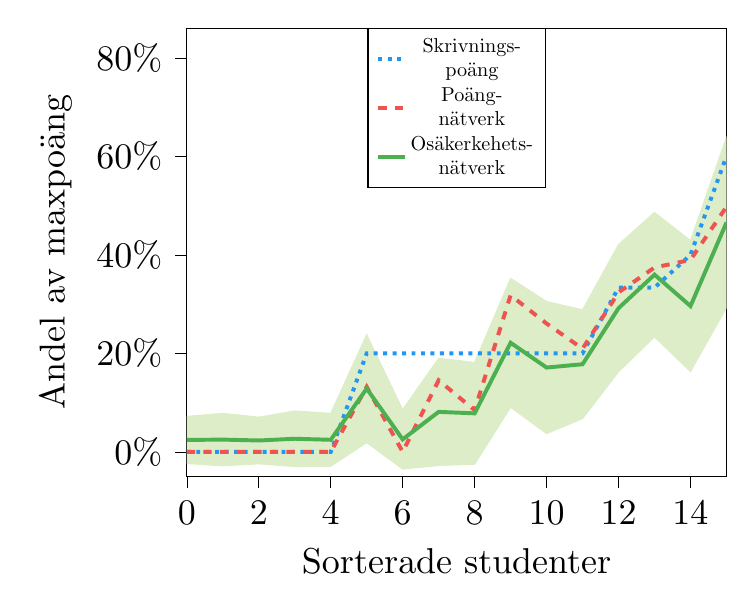
\begin{tikzpicture}

\definecolor{klight_green_100}{RGB}{220, 237, 200}
\definecolor{klight_green_200}{RGB}{197, 225, 165}
\definecolor{klight_green_300}{RGB}{174, 213, 129}
\definecolor{klight_green_400}{RGB}{156, 204, 101}
\definecolor{klight_green_500}{RGB}{139, 195, 74}
\definecolor{kred_100}{RGB}{255, 205, 210}
\definecolor{kred_400}{RGB}{239, 83, 80}
\definecolor{kyellow_400}{RGB}{255, 238, 88}
\definecolor{kgreen_300}{RGB}{129, 199, 132}
\definecolor{kgreen_500}{RGB}{76, 175, 80}
\definecolor{kblue_500}{RGB}{33, 150, 243}
\definecolor{kgrey}{RGB}{222,222,222}
\definecolor{korange}{RGB}{255, 152, 0}  % orange 500

\begin{axis}[
tick align=outside,
tick pos=left,
x grid style={white!69.01960784313725!black},
xlabel={Sorterade studenter},
xmin=0, xmax=15,
xtick style={color=black},
y grid style={white!69.01960784313725!black},
yticklabel={\pgfmathparse{\tick}\pgfmathprintnumber{\pgfmathresult}\%},
ylabel={Andel av maxpoäng},
ymin=-5, ymax=86,
legend style={at={(0.5, 1)},
                nodes={scale=0.56, transform shape},
                cells={align=center},
                anchor=north,legend columns=1},
legend image post style={scale=0.56},
ytick style={color=black},
nodes={scale=1.3, transform shape}  % increase size of everything
]
\path [draw=klight_green_100, fill=klight_green_100]
(axis cs:0,7.19785356521606)
--(axis cs:0,-2.35466599464417)
--(axis cs:1,-2.82825946807861)
--(axis cs:2,-2.41815090179443)
--(axis cs:3,-2.9727840423584)
--(axis cs:4,-2.91233801841736)
--(axis cs:5,1.88925659656525)
--(axis cs:6,-3.49166631698608)
--(axis cs:7,-2.75624513626099)
--(axis cs:8,-2.5035834312439)
--(axis cs:9,9.06870365142822)
--(axis cs:10,3.7168390750885)
--(axis cs:11,6.75616073608398)
--(axis cs:12,16.2510643005371)
--(axis cs:13,23.3353538513184)
--(axis cs:14,16.3113689422607)
--(axis cs:15,29.2561264038086)
--(axis cs:15,63.8431854248047)
--(axis cs:15,63.8431854248047)
--(axis cs:14,42.8807029724121)
--(axis cs:13,48.6091918945312)
--(axis cs:12,42.0914421081543)
--(axis cs:11,28.8315448760986)
--(axis cs:10,30.5202674865723)
--(axis cs:9,35.2254104614258)
--(axis cs:8,18.1475505828857)
--(axis cs:7,19.0004501342773)
--(axis cs:6,8.57196044921875)
--(axis cs:5,23.8038082122803)
--(axis cs:4,7.8184380531311)
--(axis cs:3,8.30120658874512)
--(axis cs:2,7.04466581344604)
--(axis cs:1,7.81208992004395)
--(axis cs:0,7.19785356521606)
--cycle;

\addplot [thick, kblue_500, line width=0.5mm, dotted]
table {%
0 0
1 0
2 0
3 0
4 0
5 20
6 20
7 20
8 20
9 20
10 20
11 20
12 33.3333320617676
13 33.3333320617676
14 40
15 60
};
\addplot [thick, kred_400, line width=0.5mm, dashed]
table {%
0 0
1 0
2 0
3 0
4 0
5 13.2092523574829
6 0
7 14.5260391235352
8 8.46072864532471
9 31.7978687286377
10 26.0492153167725
11 20.9490261077881
12 32.3769836425781
13 37.429126739502
14 38.9699935913086
15 49.7487983703613
};
\addplot [thick, kgreen_500, line width=0.5mm]
table {%
0 2.42159390449524
1 2.49191522598267
2 2.31325745582581
3 2.66421103477478
4 2.45305013656616
5 12.8465328216553
6 2.54014730453491
7 8.12210273742676
8 7.82198429107666
9 22.1470565795898
10 17.1185512542725
11 17.793851852417
12 29.1712532043457
13 35.9722747802734
14 29.5960350036621
15 46.5496559143066
};
\legend{Skrivnings-\\poäng, Poäng-\\nätverk, Osäkerkehets-\\nätverk}
\end{axis}

\end{tikzpicture}
        }
        \label{fig:un_ffm521}
    }
    \hfill
    \subfloat[Kurs B]{%
        \resizebox {0.49\textwidth}{!}{%
            % This file was created by matplotlib2tikz v0.7.4.
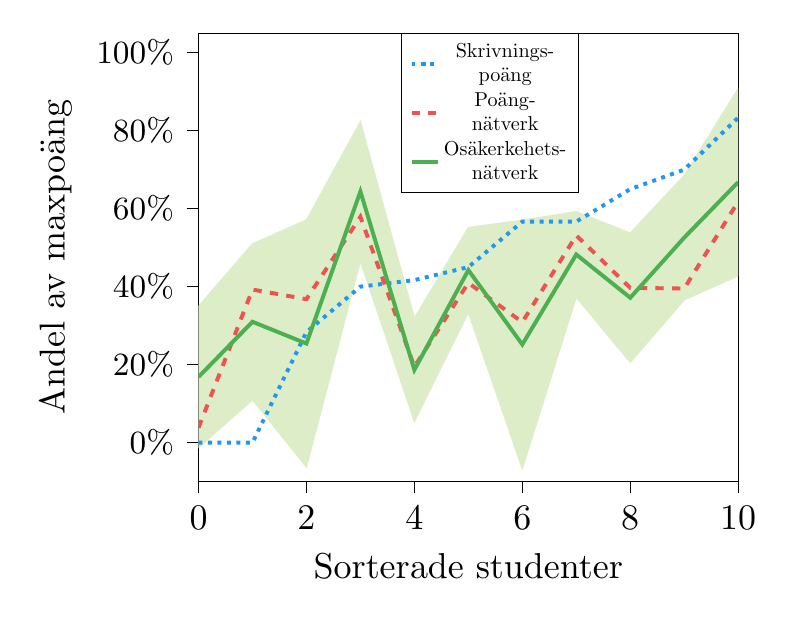
\begin{tikzpicture}

\definecolor{klight_green_100}{RGB}{220, 237, 200}
\definecolor{klight_green_200}{RGB}{197, 225, 165}
\definecolor{klight_green_300}{RGB}{174, 213, 129}
\definecolor{klight_green_400}{RGB}{156, 204, 101}
\definecolor{klight_green_500}{RGB}{139, 195, 74}
\definecolor{kred_100}{RGB}{255, 205, 210}
\definecolor{kred_400}{RGB}{239, 83, 80}
\definecolor{kyellow_400}{RGB}{255, 238, 88}
\definecolor{kgreen_300}{RGB}{129, 199, 132}
\definecolor{kgreen_500}{RGB}{76, 175, 80}
\definecolor{kblue_500}{RGB}{33, 150, 243}
\definecolor{kgrey}{RGB}{222,222,222}
\definecolor{korange}{RGB}{255, 152, 0}  % orange 500

\begin{axis}[
tick align=outside,
tick pos=left,
x grid style={white!69.01960784313725!black},
xlabel={Sorterade studenter},
xmin=0, xmax=10,
xtick style={color=black},
y grid style={white!69.01960784313725!black},
yticklabel={\small \pgfmathparse{\tick}\pgfmathprintnumber{\pgfmathresult}\%},
ylabel={Andel av maxpoäng},
ymin=-10, ymax=105,
legend style={at={(0.54, 1)},
                nodes={scale=0.56, transform shape},
                cells={align=center},
                anchor=north,legend columns=1},
legend image post style={scale=0.56},
ytick style={color=black},
nodes={scale=1.3, transform shape}  % increase size of everything
]
\path [draw=klight_green_100, fill=klight_green_100]
(axis cs:0,34.9928359985352)
--(axis cs:0,-1.3383960723877)
--(axis cs:1,10.9745483398438)
--(axis cs:2,-6.31101274490356)
--(axis cs:3,46.4410629272461)
--(axis cs:4,5.34442090988159)
--(axis cs:5,33.2976188659668)
--(axis cs:6,-6.75538206100464)
--(axis cs:7,37.2455825805664)
--(axis cs:8,20.5299205780029)
--(axis cs:9,36.5837287902832)
--(axis cs:10,42.7599716186523)
--(axis cs:10,90.8275680541992)
--(axis cs:10,90.8275680541992)
--(axis cs:9,68.5309524536133)
--(axis cs:8,53.7537307739258)
--(axis cs:7,59.2476463317871)
--(axis cs:6,57.0685577392578)
--(axis cs:5,55.1704902648926)
--(axis cs:4,31.9400272369385)
--(axis cs:3,82.3497467041016)
--(axis cs:2,57.1025199890137)
--(axis cs:1,50.9802436828613)
--(axis cs:0,34.9928359985352)
--cycle;

\addplot [thick, kblue_500, line width=0.5mm, dotted]
table {%
0 0
1 0
2 28.3333320617676
3 40
4 41.6666641235352
5 45
6 56.6666641235352
7 56.6666641235352
8 65
9 70
10 83.3333282470703
};
\addplot [thick, kred_400, line width=0.5mm, dashed]
table {%
0 3.78471374511719
1 39.2401542663574
2 36.7768135070801
3 57.9053344726562
4 19.4248161315918
5 40.9549293518066
6 30.8860702514648
7 53.1338424682617
8 39.6762275695801
9 39.505989074707
10 61.7939949035645
};
\addplot [thick, kgreen_500, line width=0.5mm]
table {%
0 16.827220916748
1 30.9773941040039
2 25.395751953125
3 64.3954086303711
4 18.6422233581543
5 44.2340545654297
6 25.156587600708
7 48.2466163635254
8 37.1418228149414
9 52.5573387145996
10 66.7937698364258
};
\legend{Skrivnings-\\poäng, Poäng-\\nätverk, Osäkerkehets-\\nätverk}
\end{axis}

\end{tikzpicture}
        }
        \label{fig:un_ffm234}
    }
    \caption{Skrivningspoäng (blå streckad) och förutsagd skrivningspoäng enligt poängnätverket (röd streckad) och osäkerhetsnätverket (grön heldragen) för en representativ valideringsmängd bestående av 15 och elva studenter i kurs A respektive B. Det grönskuggade området motsvarar en standardavvikelse för den aleatoriska osäkerheten, $\sigma_x$.}
    \label{fig:exam_score_results}
\end{figure}
En iteration av valideringsmetoden för poängnätverket och osäkerhetsnätverket för kurs A visas i figur \ref{fig:un_ffm521}. Vi noterar för den specifika iterationen att poängnätverket och osäkerhetsnätverket genererar liknande förutsägelser. För 25 iterationer presterar poängnätverket förutsägelser med ett medelabsolutfel $E = \frac{1}{N}\sum_{i=1}^N \left|y_i - \hat{y}_i\right| = 12 \pm 14\,\rm \%$. Motsvarande osäkerhetsnätverk åstadkommer förutsägelser med ett medelabsolutfel $E = 11 \pm 12\,\rm \%$. Den aleatoriska osäkerheten uppskattas av osäkerhetsnätverket till $\sigma_x = 13 \pm 9\,\rm \%$. Vi observerar därmed att för kurs A generar poängnätverket och osäkerhetsnätverket förutsägelser med jämförbara medelabsolutfel: $E = 12 \pm 14\,\rm \%$ respektive $E = 11 \pm 12\,\rm \%$.

Vidare presenteras en iteration av valideringsmetoden för kurs B i figur \ref{fig:un_ffm234}. Likt i figur \ref{fig:un_ffm521} åstadkommer poängnätverket och osäkerhetsnätverket för kurs B jämförbara förutsägelser för iterationen. För kurs B och 25 iterationer i valideringsmetoden ger poängnätverket förutsägelser med ett medelabsolutfel $E = 17 \pm 8\,\rm \%$ och osäkerhetsnätverket ett medelabsolutfel $E = 18 \pm 14\,\rm \%$. Osäkerhetsnätverket uppskattar den aleatoriska osäkerheten till $\sigma_x = 17 \pm 11\,\rm \%$. Likt kurs A noterar vi att poängnätverket och osäkerhetsnätverket åstadkommer förutsägelser med liknande medelabsolutfel: $E = 17 \pm 13\,\rm \%$ och $E = 18 \pm 14\,\rm \%$.

Jämförelsevis noterar vi att motsvarande medelabsolutfel för kurs B är fem till sex procentenheter större än i kurs A. Dessutom är även uppskattningen av den aleatoriska osäkerheten mindre för kurs A än för kurs B. För kurs A är $\sigma_x = 13 \pm 9\,\rm \%$ medan för kurs B är $\sigma_x = 17 \pm 11 \,\rm \%$. Att nätverken presterar bättre i kurs A än i kurs B är i linje med observationen att U/G- och U/5-nätverken genererar högre träffsäkerheter i kurs A än kurs B. Därtill noterar vi en likhet mellan de två kurserna. Likheten är att osäkerhetsnätverken presterar jämförbart med poängnätverken. För kurs A och kurs B har därmed den aleatoriska osäkerheten för skrivningspoängsproblemet uppskattats utan större försämringar i medelabsolutfelet.

Notera att de uppskattade aleatoriska osäkerheterna inte ska tolkas som direkta osäkerheter i förutsägelserna. Som introducerades i avsnitt \ref{NN_and_uncert} utgör $\sigma_x$ en av komponenterna för att uppskatta förutsägelserosäkerheten $\sigma_y = U(\sigma_x, \sigma_W)$ i kombination med den epistemiska osäkerheten $\sigma_W$ och en funktion $U$. Eftersom $\sigma_x$ har införts utan större försämringar i medelabsolutfel finns det ett värde i att försöka införa $\sigma_W$ och $U$ i ett fortsatt arbete för att uppskatta $\sigma_y$.

%Det är även möjligt att observera ett potentiellt samband mellan kursernas medelabsolutfel och uppskattade aleatoriska osäkerheter. För kurs A gäller $E / \sigma_x = 0.85$ och kurs B $E / \sigma_x = 1.07$, vilket spekulativt kan indikera på ett samband $E / \sigma_x = 1$.


%\textbf{Förbättringspunkt: Kvantifiera hur väl den aleatoriska osäkerheten överensstämmer med den verkliga osäkerheten?}

%\textbf{Förklaringar till varför resultaten är bättre för FFM521: 1. Mer data och 2. bonusuppgifter i kursen.}

\subsection{Sammanfattande diskussion}
\label{sec:Deep-D}
Nedan följer en sammanfattande diskussion om utvecklingen av djupinlärningsalgoritmer för att förutsäga studieresultat och modellera osäkerheter. Först identifieras en möjlig förbättring av datarepresentationen. Därefter diskuteras effekten av den noterade låga datamängden och möjligheterna som en större datamängd kan medföra. 

I avsnitt \ref{sec:error_analysis} noteras att både U/G-nätverket och U/5-nätverket har en högre träffsäkerhet i klassificeringen av underkända än godkända studenter. I kurs A kan skillnaden förklaras av en överrepresentation av underkända studenter för både U/G- och U/5-problemet. Förklaringen håller dock inte för kurs B, då underkända studenter endast är överrepresenterade för U/5-problemet. Överrepresentation är därmed inte en heltäckande förklaring. En annan aspekt som kan bidra till skillnaden är de förvalda värdena i våra tensorer, vilka i allmänhet framhäver underkända studenter. En möjlig förbättring kan därav vara en justering av de förvalda värdena sådan att de underkända studenterna inte viktas i lika stor utsträckning. Potentiellt kan justeringen leda till att den övergripande träffsäkerheten för både U/G-problemet och U/5-problemet förbättras.

Den totala träffsäkerheten kan även påverkas av storleken på datamängden. Vi noterade i sektion \ref{sec:DDD} att den tillgängliga datamängden är relativt begränsad, vilket också framgår i våra resultat beskrivna i sektion \ref{sec:results_ug_u5} och \ref{sec:uncert}. Till exempel är träffsäkerheten för både U/G-problemet och U/5-problemet högre i kurs A än kurs B, där datamängden är över $50 \, \%$ större. Dessutom är medelabsolutfelet för förutsägelserna från poäng- och osäkerhetsnätverken mindre i kurs A än kurs B. En konsekvens av en större datamängd kan alltså vara en högre träffsäkerhet och ett mindre medelabsolutfel. Träffsäkerheterna är även känsliga för blandningen av datan och kan ses i de relativt stora standardavvikelserna från valideringsmetoden.

Vi ser primärt två metoder för att öka datamängden. Den ena metoden är att samla in data från samma kurs under flera år. Nackdelen med att endast använda data från samma kurs är att det begränsar möjligheten att undersöka hur nätverken generaliserar till andra kurser.  Den andra metoden är att bredda dataninsamlingen till fler kurser, men i nuläget stödjer inte våra resultat att konkatenering från flera kurser leder till förbättrade träffsäkerheter.

Även om träffsäkerheterna för konkatenering är lägre än för enskilda kurser observerar vi indikationer på att det finns vissa gemensamma mönster mellan kurs A och B. I avsnitt \ref{sec:results_ug_u5} observerade vi att U/G-nätverket presterar bättre och att U/5-nätverket presterar något sämre än baslinjen vid träning på all data i en kurs och test på den andra. Utifrån våra resultat kan vi därmed dra slutsatsen att viss generalisering sker, men inte i tillräckligt stor utsträckningen för att överträffa träffsäkerheten som uppnås med data från samma kurs. Vi identifierar därför ett generaliseringsproblem som behöver lösas för att till fullo dra nytta av en utökad datamängd från en bredd av fler kurser. 

För att angripa generaliseringsproblemet finns det utarbetade strategier inom djupinlärning. Exempelvis inom textanalys och bildigenkänning är en vanlig metod att träna neurala nätverk i två steg \cite{Chollet}. Förenklat tränas först en bas av nätverket på generell data, varefter basens vikter fixeras och den återstående delen av nätverket tränas på specifik data.
En annan möjlig metod är att utnyttja att datan över studiemönstren är en tidsserie. Rekursiva neurala nätverk, som långt-korttidsminnesnätverk. (eng. \emph{long short-term memory}) \cite{Chollet} är generellt lämpade för tidsserier. Emellertid kräver långt-korttidsminnesnätverk generellt stora datamängder och våra preliminära försök med dessa har hittills varit fruktlösa. 

% Ytterligare noterar vi att osäkerhetsnätverkens uppskattningar av den aleatoriska osäkerheten är mindre för kurs A med en större datamängd än kurs B. På samma sätt att en större datamängd kan ge ett lägre medelabsolutfel för osäkerhetsnätverken, kan mer data resultera i lägre uppskattade aleatoriska osäkerheter. Minskningen i osäkerhet kan rimliggöras genom ekvation \eqref{eq:loss_fcn} eftersom ett minskat förutsägelsefel $\left\|y - f^\mathbf{W}(\mathbf{x})\right\|_2$ möjliggör för en minskad osäkerhetsattenuation $\exp{\left(-\log \sigma_x^2 \right)}$.

Oberoende av större datamängder visar osäkerhetsnätverken att den aleatoriska osäkerheten för skrivningspoängsproblemet kan uppskattas utan större försämringar i medelabsolutfel. Våra resultat med att införa den aleatoriska osäkerheten kan motivera vidare studier om att modellera osäkerheter i förutsägelsen av studieresultat. Ett möjligt nästa steg vore därför att införa den aleatoriska osäkerheten i U/G-nätverken och U/5-nätverken. Detta skulle ge möjligheten att bortse ifrån förutsägelser vid stor osäkerhet. Därmed är det möjligt att undvika felaktiga förutsägelser och därav höja träffsäkerheten. Ett annat möjligt nästa steg är att inkludera den epistemiska osäkerheten för att förbättra modelleringen av förutsägelseosäkerheterna. I en sådan utvecklingsprocess behövs en analys av i vilken utsträckning de modellerade osäkerheterna överensstämmer med förutsägelsernas verkliga osäkerheter.

Sammanfattningsvis har vi i detta kapitel visat hur djupinlärning kan användas för att förutsäga studenters studieresultat med god träffsäkerhet, speciellt för problemet att förutsäga underkänt eller godkänt. För skrivningspoängsproblemet har vi visat att aleatorisk osäkerhet kan införas utan en större försämring av medelabsolutfel. Med detta sagt finns flera utvecklingsområden, exempelvis har vi identifierat generalisingsproblemet och införandet av den aleatoriska osäkerheten för U/G- och för U/5-problemet. Med en större datamängd bedömer vi att generaliseringsproblemet kan lösas och att de redan goda träffsäkerheterna kan förbättras ytterligare.

% \textbf{Allmänna förbättringspunkter och felkällor}

% \textbf{Liten datamängd}

% \textbf{-> Bättre generaliseringsmöjligheter (Strategier för att bygga bättre generaliseringsnetvärk)}

% \textbf{-> Bättre osäkerhetsnätverk}

% \textbf{-> Sammankoppling av osäkerhetsnätverk och förutsägelser av betyg.}

% \textbf{Resultaten är bra}

% 1. Datamängd liten
% 2. Nätverken generaliserar
% 3. Data representation
% 4. Diskussion om osäkerhetsmodellen.
% 5. Nyttan av osäkerheterna. Kan göra förutsägelser 
% 6. Hur bra är resultaten?

% Felkällor/Brister



% Förbättringspunkter
% En mer rigorös diskussion av felanalys.
% En mer jämn tensor - framhäver ingen. 